\documentclass[12pt, a4paper]{article}

\usepackage[utf8]{inputenc}
\usepackage[T1]{fontenc}
\usepackage[romanian]{babel}
\usepackage{geometry}
\geometry{a4paper, margin=2cm}
\usepackage{hyperref}
\usepackage{enumitem}
\usepackage{amsmath}
\usepackage{graphicx}
\usepackage{float}

\title{\textbf{Detecția de anomalii vizuale în producție industrială} \\ \large Documentație}
\author{Tudor-Adelin Vancea gr. 30233 s. 2}
\date{}

\begin{document}

\maketitle

\section{Introducere și Scopul Proiectului}
În industrie, detecția automată a defectelor pe liniile de producție se realizează adesea prin modele antrenate exclusiv pe exemple de piese \textit{normale}. Scopul acestui proiect este implementarea unui sistem de detecție vizuală a anomaliilor, de tip nesupervizat, folosind metode clasice de procesare a imaginilor (Classical Computer Vision), implementate manual, de la zero.

Cerințele îndeplinite:
\begin{itemize}
    \item \textbf{Antrenare/Referință:} Utilizarea imaginilor normale (fără defecte) pentru a stabili un etalon (\textit{Golden Template}).
    \item \textbf{Detecție și localizare:} Identificarea defectelor și localizarea lor printr-o hartă termică (\textit{Heatmap}) și o mască de anomalii (\textit{Anomaly Mask}).
    \item \textbf{Algoritmi Custom:} Implementarea matematică, folosind \texttt{NumPy} și operații vectorizate, fără utilizarea funcțiilor \textit{black-box} de filtrare din OpenCV.
\end{itemize}

\section{Metodologie și Algoritmi Implementați}
Procesul de detecție a anomaliilor este împărțit în mai multe etape de procesare, detaliate în funcțiile din modulul \texttt{algorithms.py}.

\subsection{Conversia în Tonuri de Gri (Grayscale)}
Pentru a simplifica procesarea, imaginile color sunt transformate în tonuri de gri. În implementare sunt propuse două abordări. Cea principală utilizează o medie simplă a canalelor:
\begin{equation}
    I_{gray} = \frac{1}{3}R + \frac{1}{3}G + \frac{1}{3}B
\end{equation}
Alternativ, se poate utiliza formula bazată pe luminozitate:
\begin{equation}
    I_{gray} = 0.299 \cdot R + 0.587 \cdot G + 0.114 \cdot B
\end{equation}

\subsection{Filtrarea Zgomotului (Filtru Gaussian)}
Pentru atenuarea zgomotului gaussian, a fost implementat manual un filtru spațial. Eliminarea zgomotului se face cu un filtru având o formă și o dimensiune $w$ adecvată, în concordanță cu deviația standard $\sigma$. Dimensiunea $w$ a kernel-ului de convoluție este aleasă aproximativ $w \approx 6\sigma$. Formula de construire a elementelor kernel-ului Gaussian $G$ este:
\begin{equation}
    G(x, y) = \frac{1}{2\pi\sigma^2} e^{-\frac{(x-x_0)^2+(y-y_0)^2}{2\sigma^2}}
\end{equation}
unde $(x_0, y_0)$ reprezintă coordonatele coloanei și liniei centrale a nucleului.

Aplicarea kernel-ului pe imagine (convoluția) este optimizată prin extragerea tuturor ferestrelor glisante folosind \texttt{sliding\_window\_view} și calcularea produsului de convoluție pe matrice (\texttt{np.tensordot}):
\begin{equation}
    I_{filtered}(i, j) = \sum_{u} \sum_{v} I_{gray}(i+u, j+v) \cdot G(u, v)
\end{equation}

\subsection{Modelul de Referință (Golden Template)}
Faza de antrenare presupune crearea unui model statistic pe baza unui set de $N$ imagini normale. Se calculează imaginea medie ($\mu$) și deviația standard per pixel ($\sigma_{template}$), care indică varianța naturală a fiecărui pixel.
\begin{equation}
    \mu = \frac{1}{N} \sum_{k=1}^{N} I_k
\end{equation}
\begin{equation}
    Var = \frac{1}{N} \sum_{k=1}^{N} (I_k - \mu)^2
\end{equation}
Prin urmare, deviația standard se obține ca rădăcină pătrată a varianței:
\begin{equation}
    \sigma_{template} = \sqrt{Var} = \sqrt{\frac{1}{N} \sum_{k=1}^{N} (I_k - \mu)^2}
\end{equation}

\subsection{Detecția Anomaliilor (Z-Score)}
Pentru a diferenția o anomalie, se calculează diferența absolută dintre imaginea de test și etalon. Inițial, pentru binarizare s-a experimentat algoritmul Otsu, însă acesta eșuează pe imagini complet normale deoarece forțează mereu împărțirea histogramei în două clase. Astfel, în lipsa unui defect real (când histograma este unimodală), Otsu secționează eronat zgomotul inofensiv de senzor și clasifică artificial o parte din el drept anomalie. Pentru a remedia acest neajuns, implementarea finală utilizează o hartă de \textbf{Z-Score}, care ține cont de deviația standard locală:
\begin{equation}
    Z = \frac{|I_{test} - \mu|}{\sigma_{template} + \epsilon}
\end{equation}
unde $\epsilon = 2.0$ este un termen de siguranță pentru evitarea împărțirii la zero. 

Această abordare este mult mai robustă deoarece raportează diferența unui pixel la variația sa obișnuită (înregistrată în faza de antrenare). Dacă un pixel are o deviație standard mare, înseamnă că el variază în mod natural destul de mult de-a lungul setului de antrenare, deci o diferență mare față de medie în imaginea de test va rezulta într-un scor Z mic, nefiind marcat în mod eronat ca anomalie. În schimb, pentru un pixel cu o deviație standard foarte mică (stabil în mod normal), aceeași diferență absolută va genera un scor Z foarte mare, semnalând prezența unei adevărate anomalii.

Masca inițială de anomalii este generată aplicând un prag (ex. $Z_{threshold} = 3.5$):
\begin{equation}
    Mask_{initial}(x, y) = 
    \begin{cases} 
      255, & Z(x, y) > Z_{threshold} \\
      0, & \text{altfel}
    \end{cases}
\end{equation}

\subsection{Post-procesare: Operații Morfologice}
Masca inițială poate conține zgomot (fals pozitive) sau găuri în interiorul defectelor. S-au implementat operațiile morfologice de bază folosind ferestre glisante (\textit{sliding windows}) de dimensiune $3 \times 3$. În prealabil, imaginea este extinsă („padded” cu zerouri) pentru a procesa corect și marginile.
\begin{itemize}
    \item \textbf{Eroziunea} simulează subțierea obiectelor albe luând valoarea minimă din fereastra $3 \times 3$. Dacă există cel puțin un pixel negru (0) în vecinătate, pixelul central devine 0 (eliminând zgomotul fin): 
    \begin{equation}
        (I \ominus K)(x, y) = \min_{(i,j) \in W_{3\times3}} I(x+i, y+j)
    \end{equation}
    \item \textbf{Dilatarea} îngroașă obiectele albe luând valoarea maximă din fereastra $3 \times 3$. Dacă există cel puțin un pixel alb (255) în vecinătate, pixelul central devine 255 (unind componente fragmentate):
    \begin{equation}
        (I \oplus K)(x, y) = \max_{(i,j) \in W_{3\times3}} I(x+i, y+j)
    \end{equation}
\end{itemize}
Masca finală este obținută printr-o operație de \textit{Opening} (pentru a elimina zgomotul mic) urmată de un \textit{Closing} repetat (pentru a uni fragmentele de anomalie, realizat iterativ).

\subsection{Generare Heatmap}
Pentru vizualizare, diferența absolută normalizată în intervalul $v \in [0, 1]$ este mapată într-un spațiu RGB (folosind o paletă de culori personalizată) prin următoarele ecuații pentru canale (implementate cu \texttt{np.clip}):
\begin{align}
    R(v) &= 1.5 - |4v - 3| \\
    G(v) &= 1.5 - |4v - 2| \\
    B(v) &= 1.5 - |4v - 1|
\end{align}
Rezultatele finale sunt scalate în intervalul $[0, 255]$ pentru afișare.

\section{Arhitectura Sistemului}
Proiectul menține o arhitectură modulară:
\begin{itemize}
    \item \texttt{algorithms.py}: Conține toate implementările matematice (Z-score, convoluții, filtre, morfologie, LUT heatmap).
    \item \texttt{data\_loader.py}: Se ocupă de încărcarea și partiționarea fișierelor din dataset.
    \item \texttt{pipeline.py}: Fluxul principal (\textit{interactive pipeline}), bazat pe o interfață CLI și \texttt{tkinter} pentru selecția fișierelor, vizualizând comparativ imaginile cu \texttt{OpenCV} (Original, Etalon, Heatmap, Mască finală).
\end{itemize}

\section{Imagini și Rezultate (Runtime)}
Această secțiune este rezervată pentru adăugarea vizuală a rezultatelor execuției programului. Se vor adăuga capturi de ecran cuprinzând imaginea de test originală, template-ul mediu, harta termică și masca finală obținută, pentru diferite categorii de obiecte (ex. \textit{Bottle, Wood, Hazelnut}, etc.).

\subsection{Bottle}
\begin{figure}[H]
    \centering
    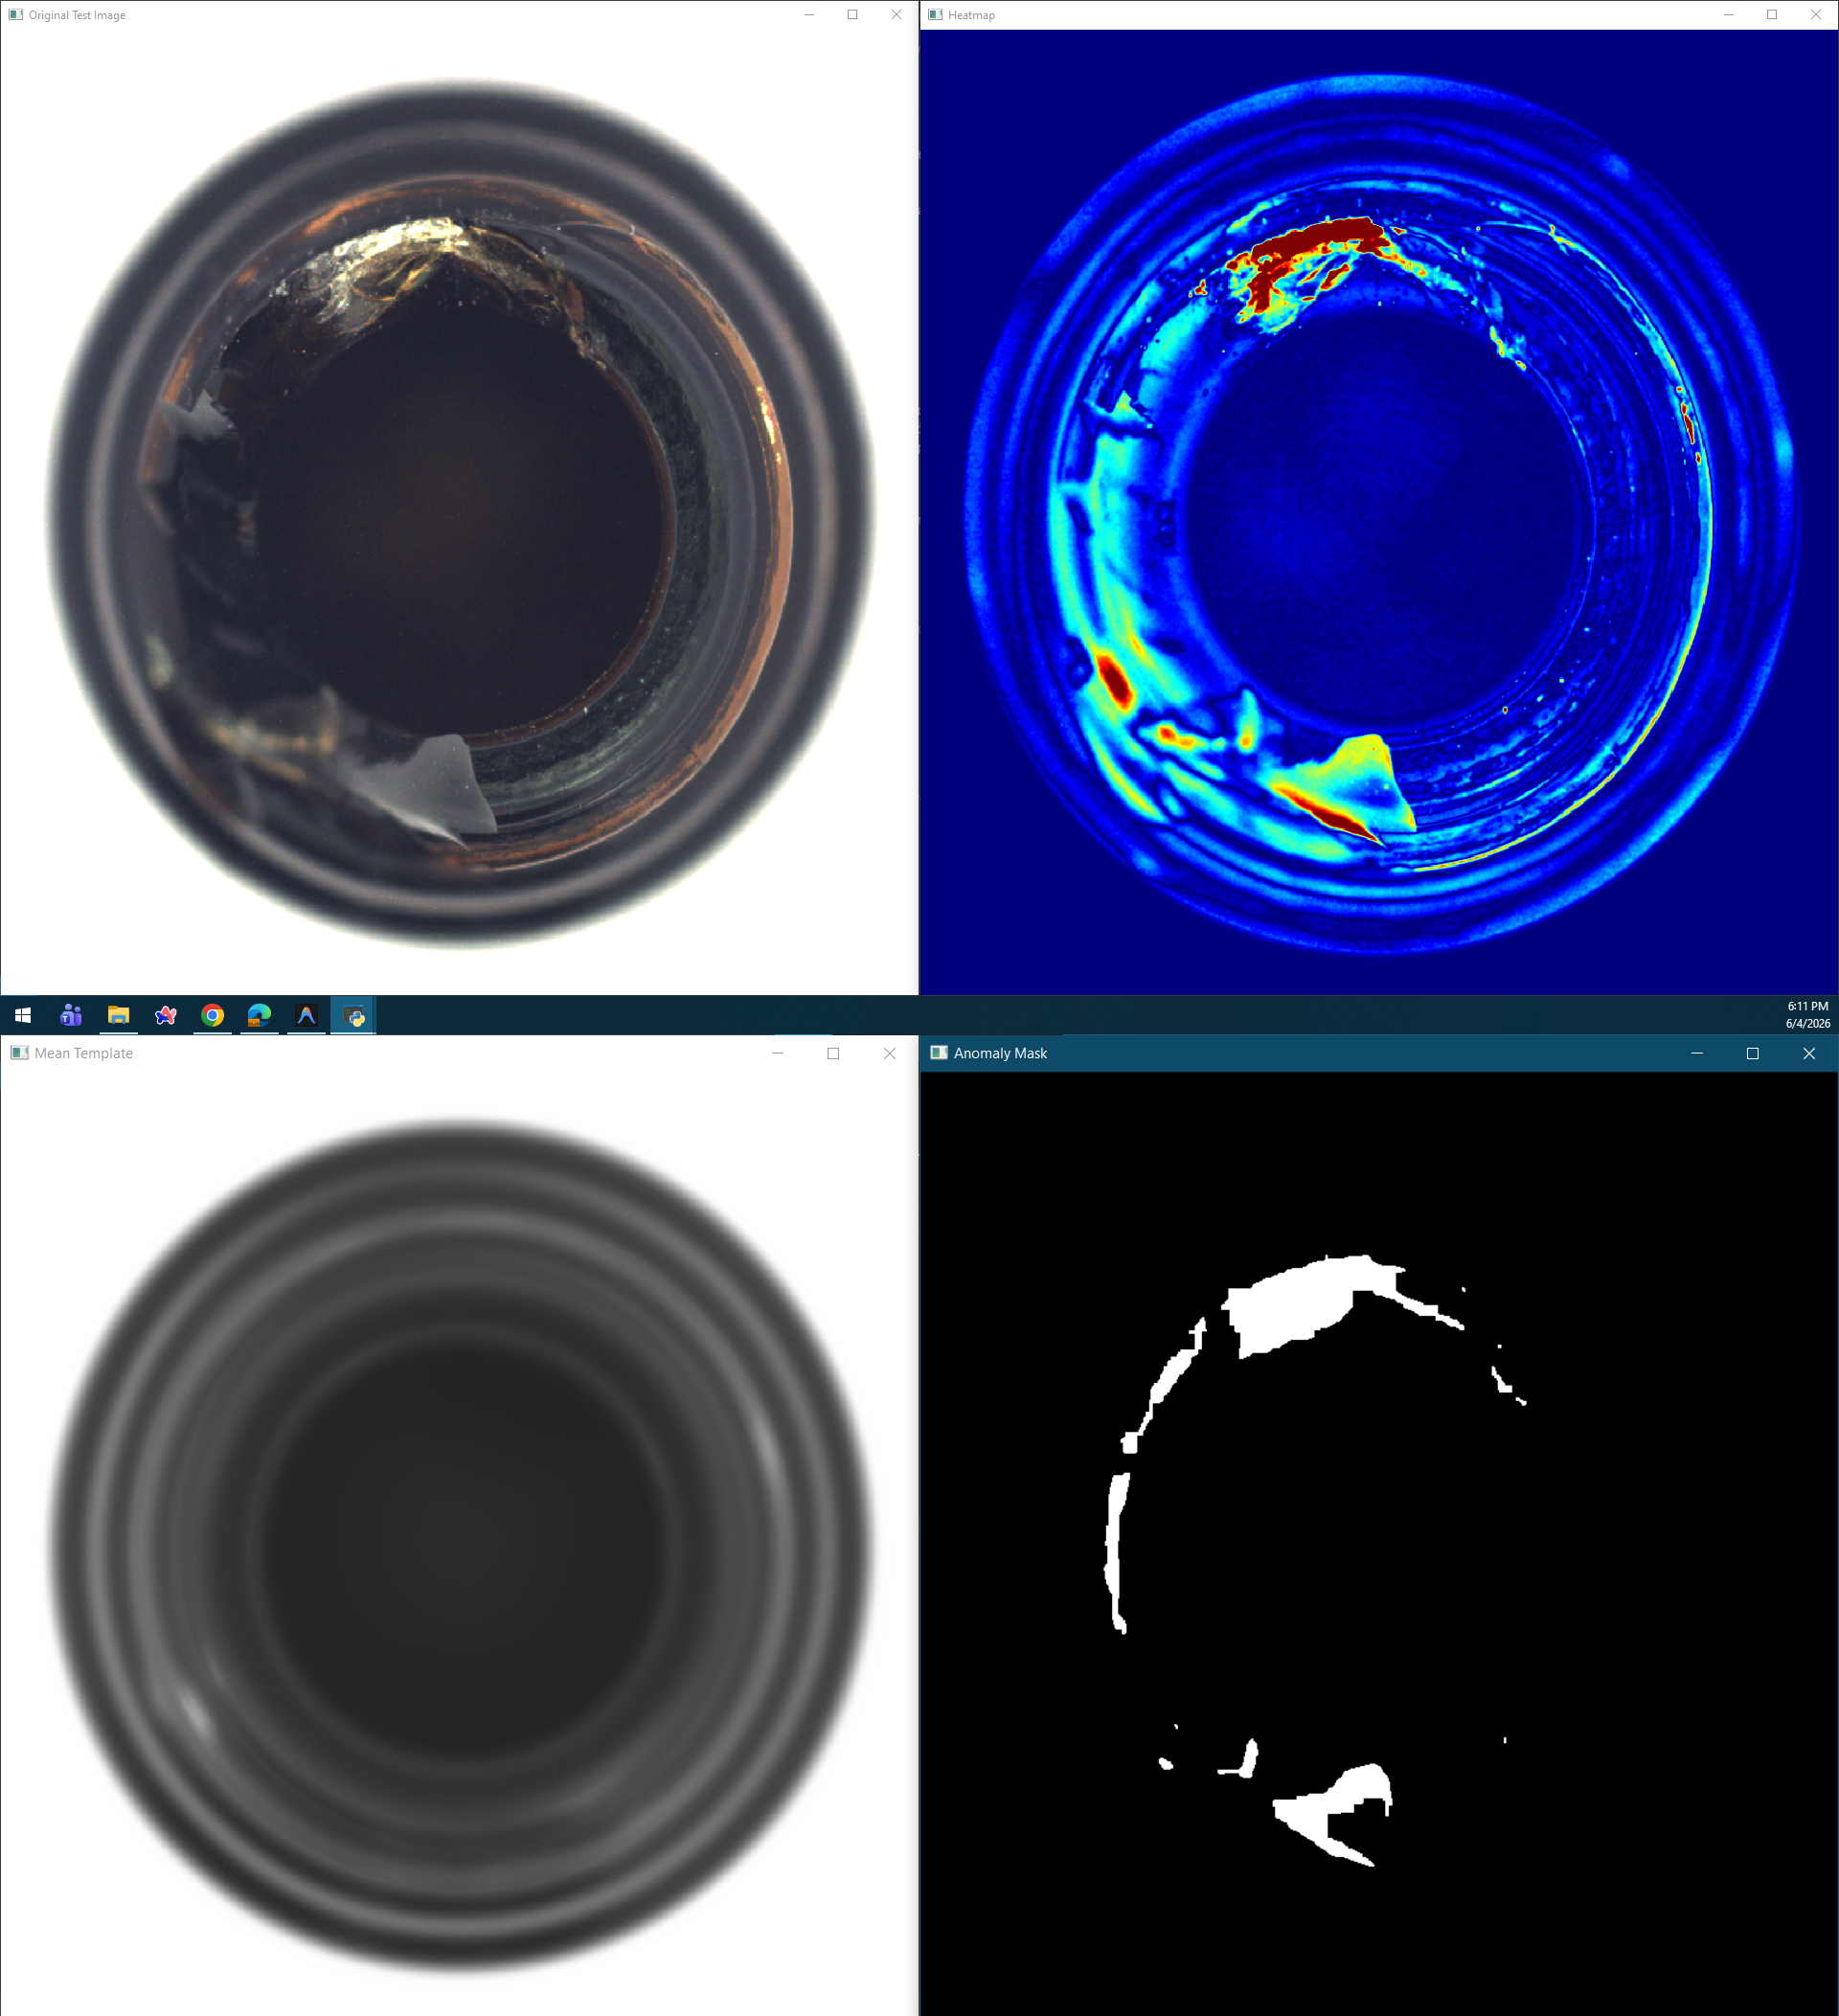
\includegraphics[width=0.8\textwidth]{runtime-images/bottle/bottle-broken-large-result18.png}
    \caption{Bottle: bottle-broken-large-result18.png}
\end{figure}

\begin{figure}[H]
    \centering
    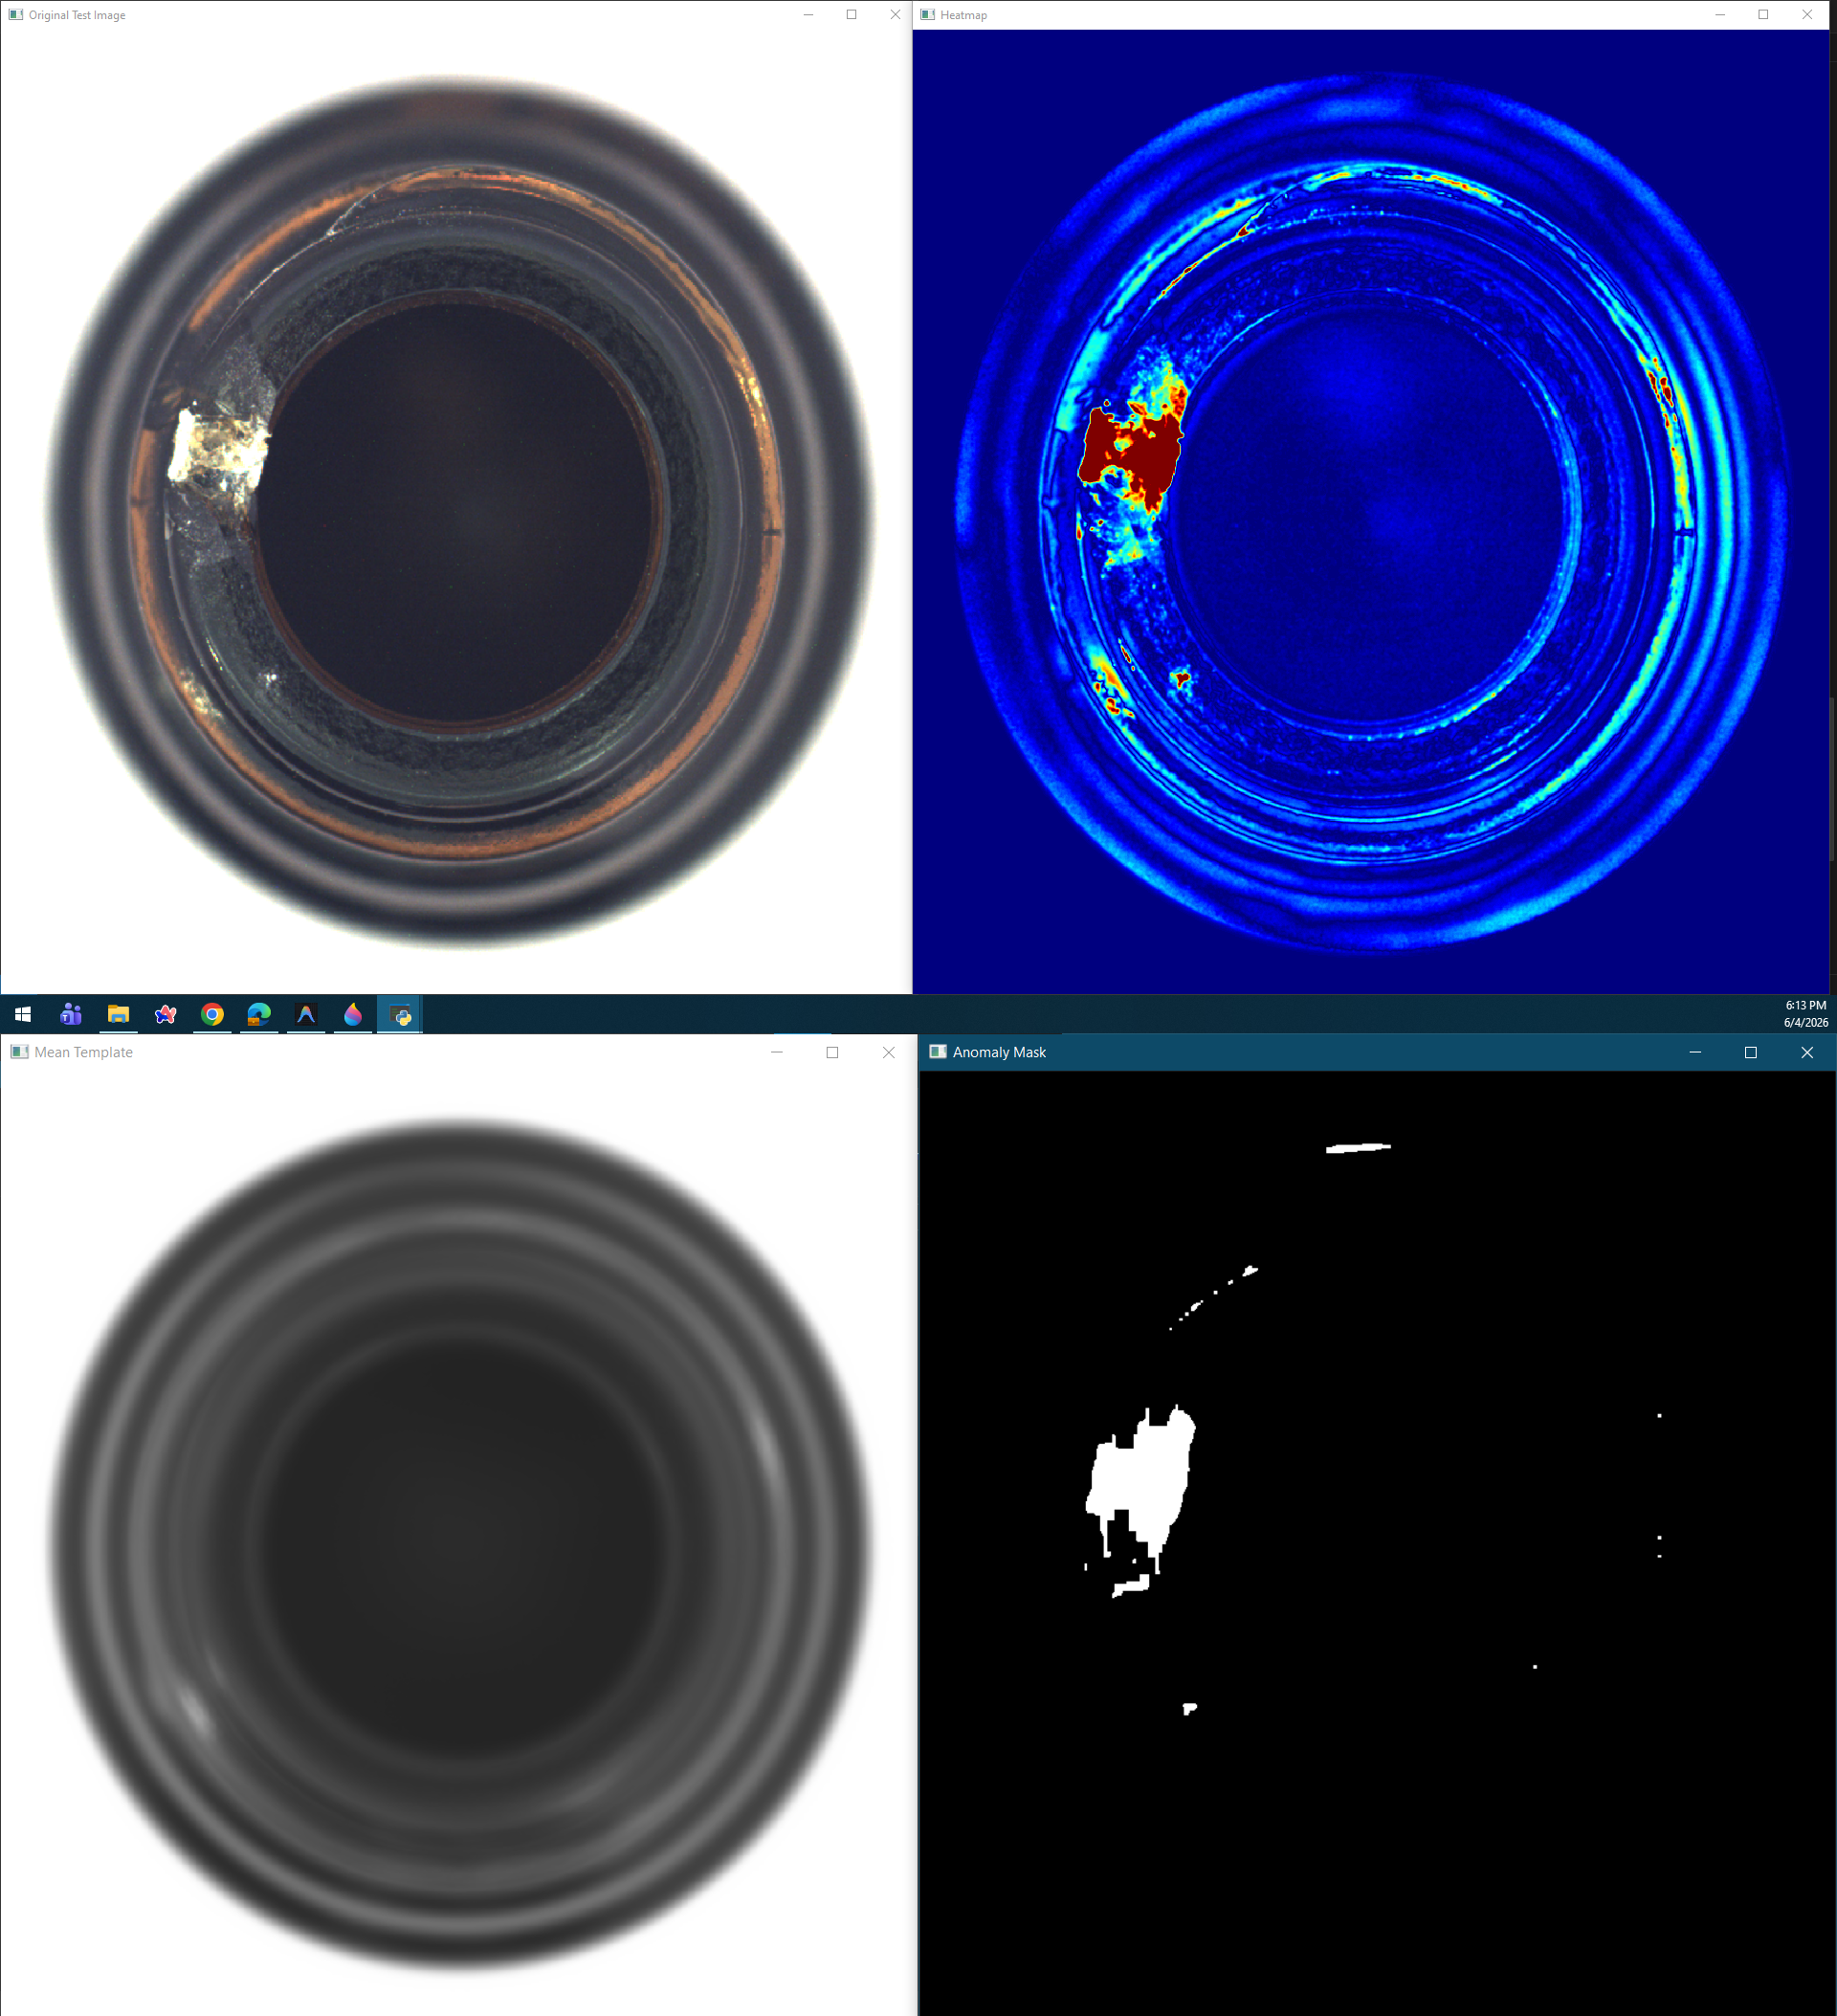
\includegraphics[width=0.8\textwidth]{runtime-images/bottle/bottle-broken-small-result17.png}
    \caption{Bottle: bottle-broken-small-result17.png}
\end{figure}

\begin{figure}[H]
    \centering
    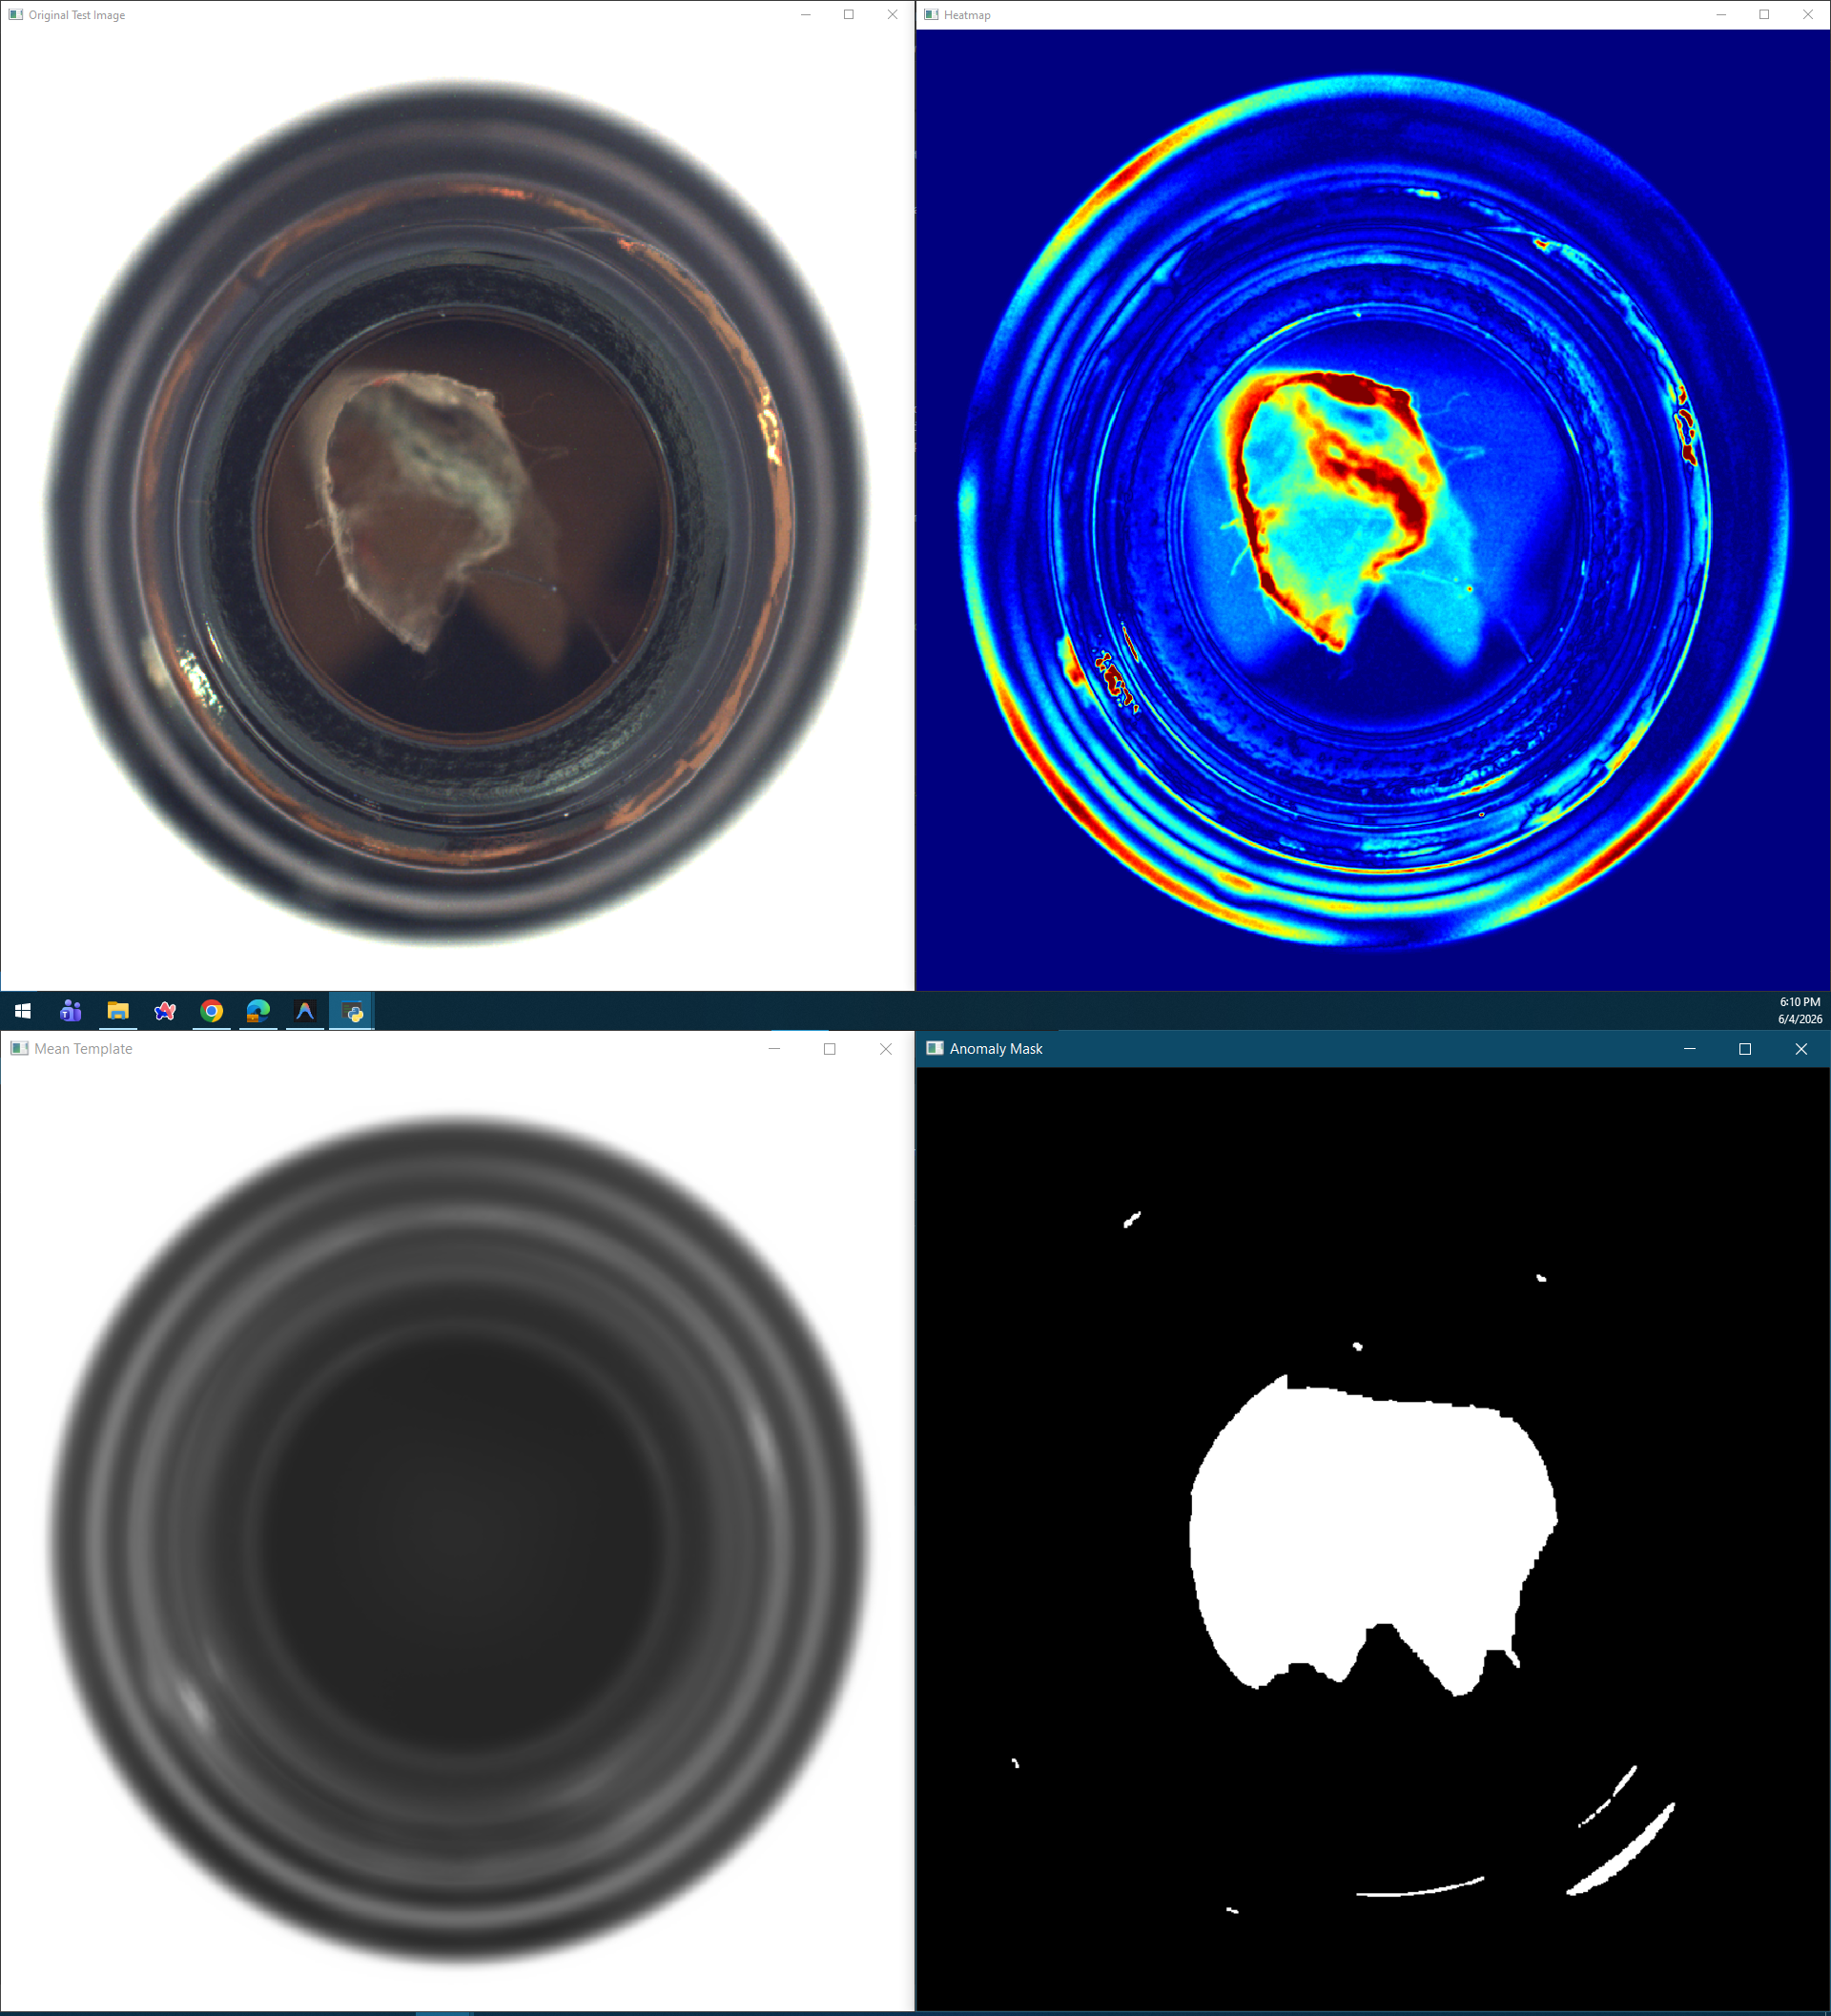
\includegraphics[width=0.8\textwidth]{runtime-images/bottle/bottle-contamination-result5.png}
    \caption{Bottle: bottle-contamination-result5.png}
\end{figure}

\begin{figure}[H]
    \centering
    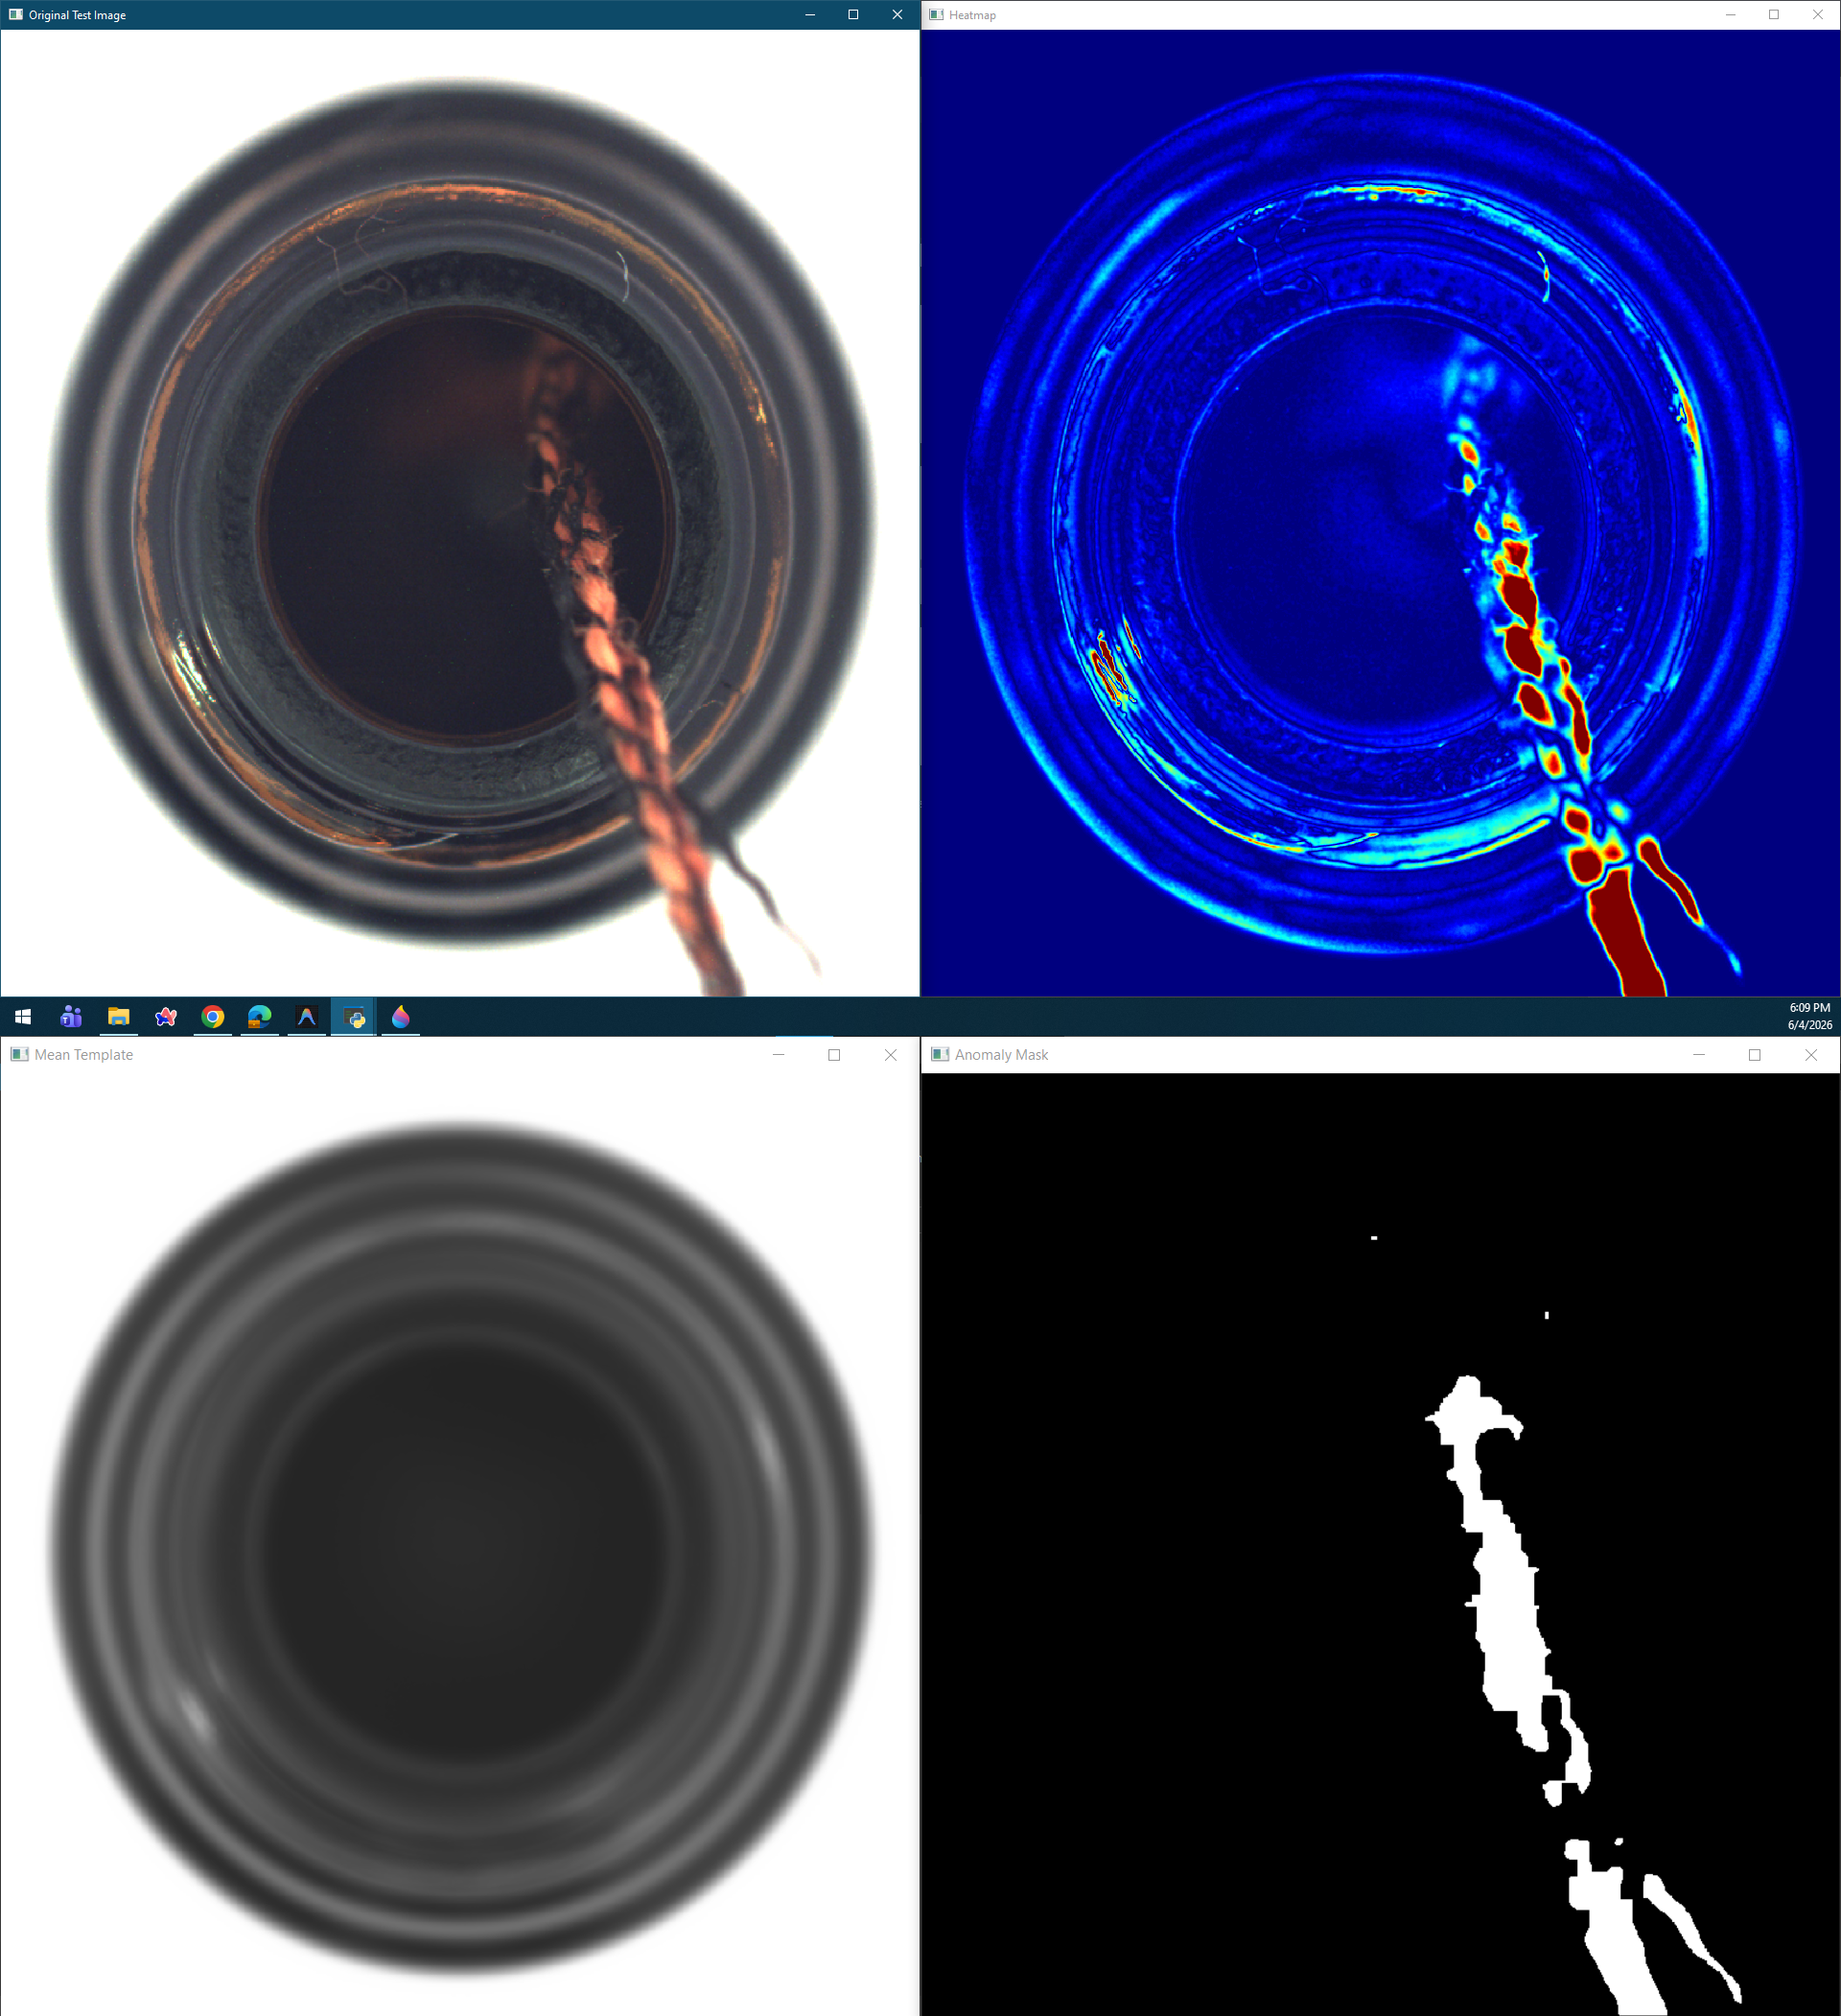
\includegraphics[width=0.8\textwidth]{runtime-images/bottle/bottle-contamination-result7.png}
    \caption{Bottle: bottle-contamination-result7.png}
\end{figure}

\begin{figure}[H]
    \centering
    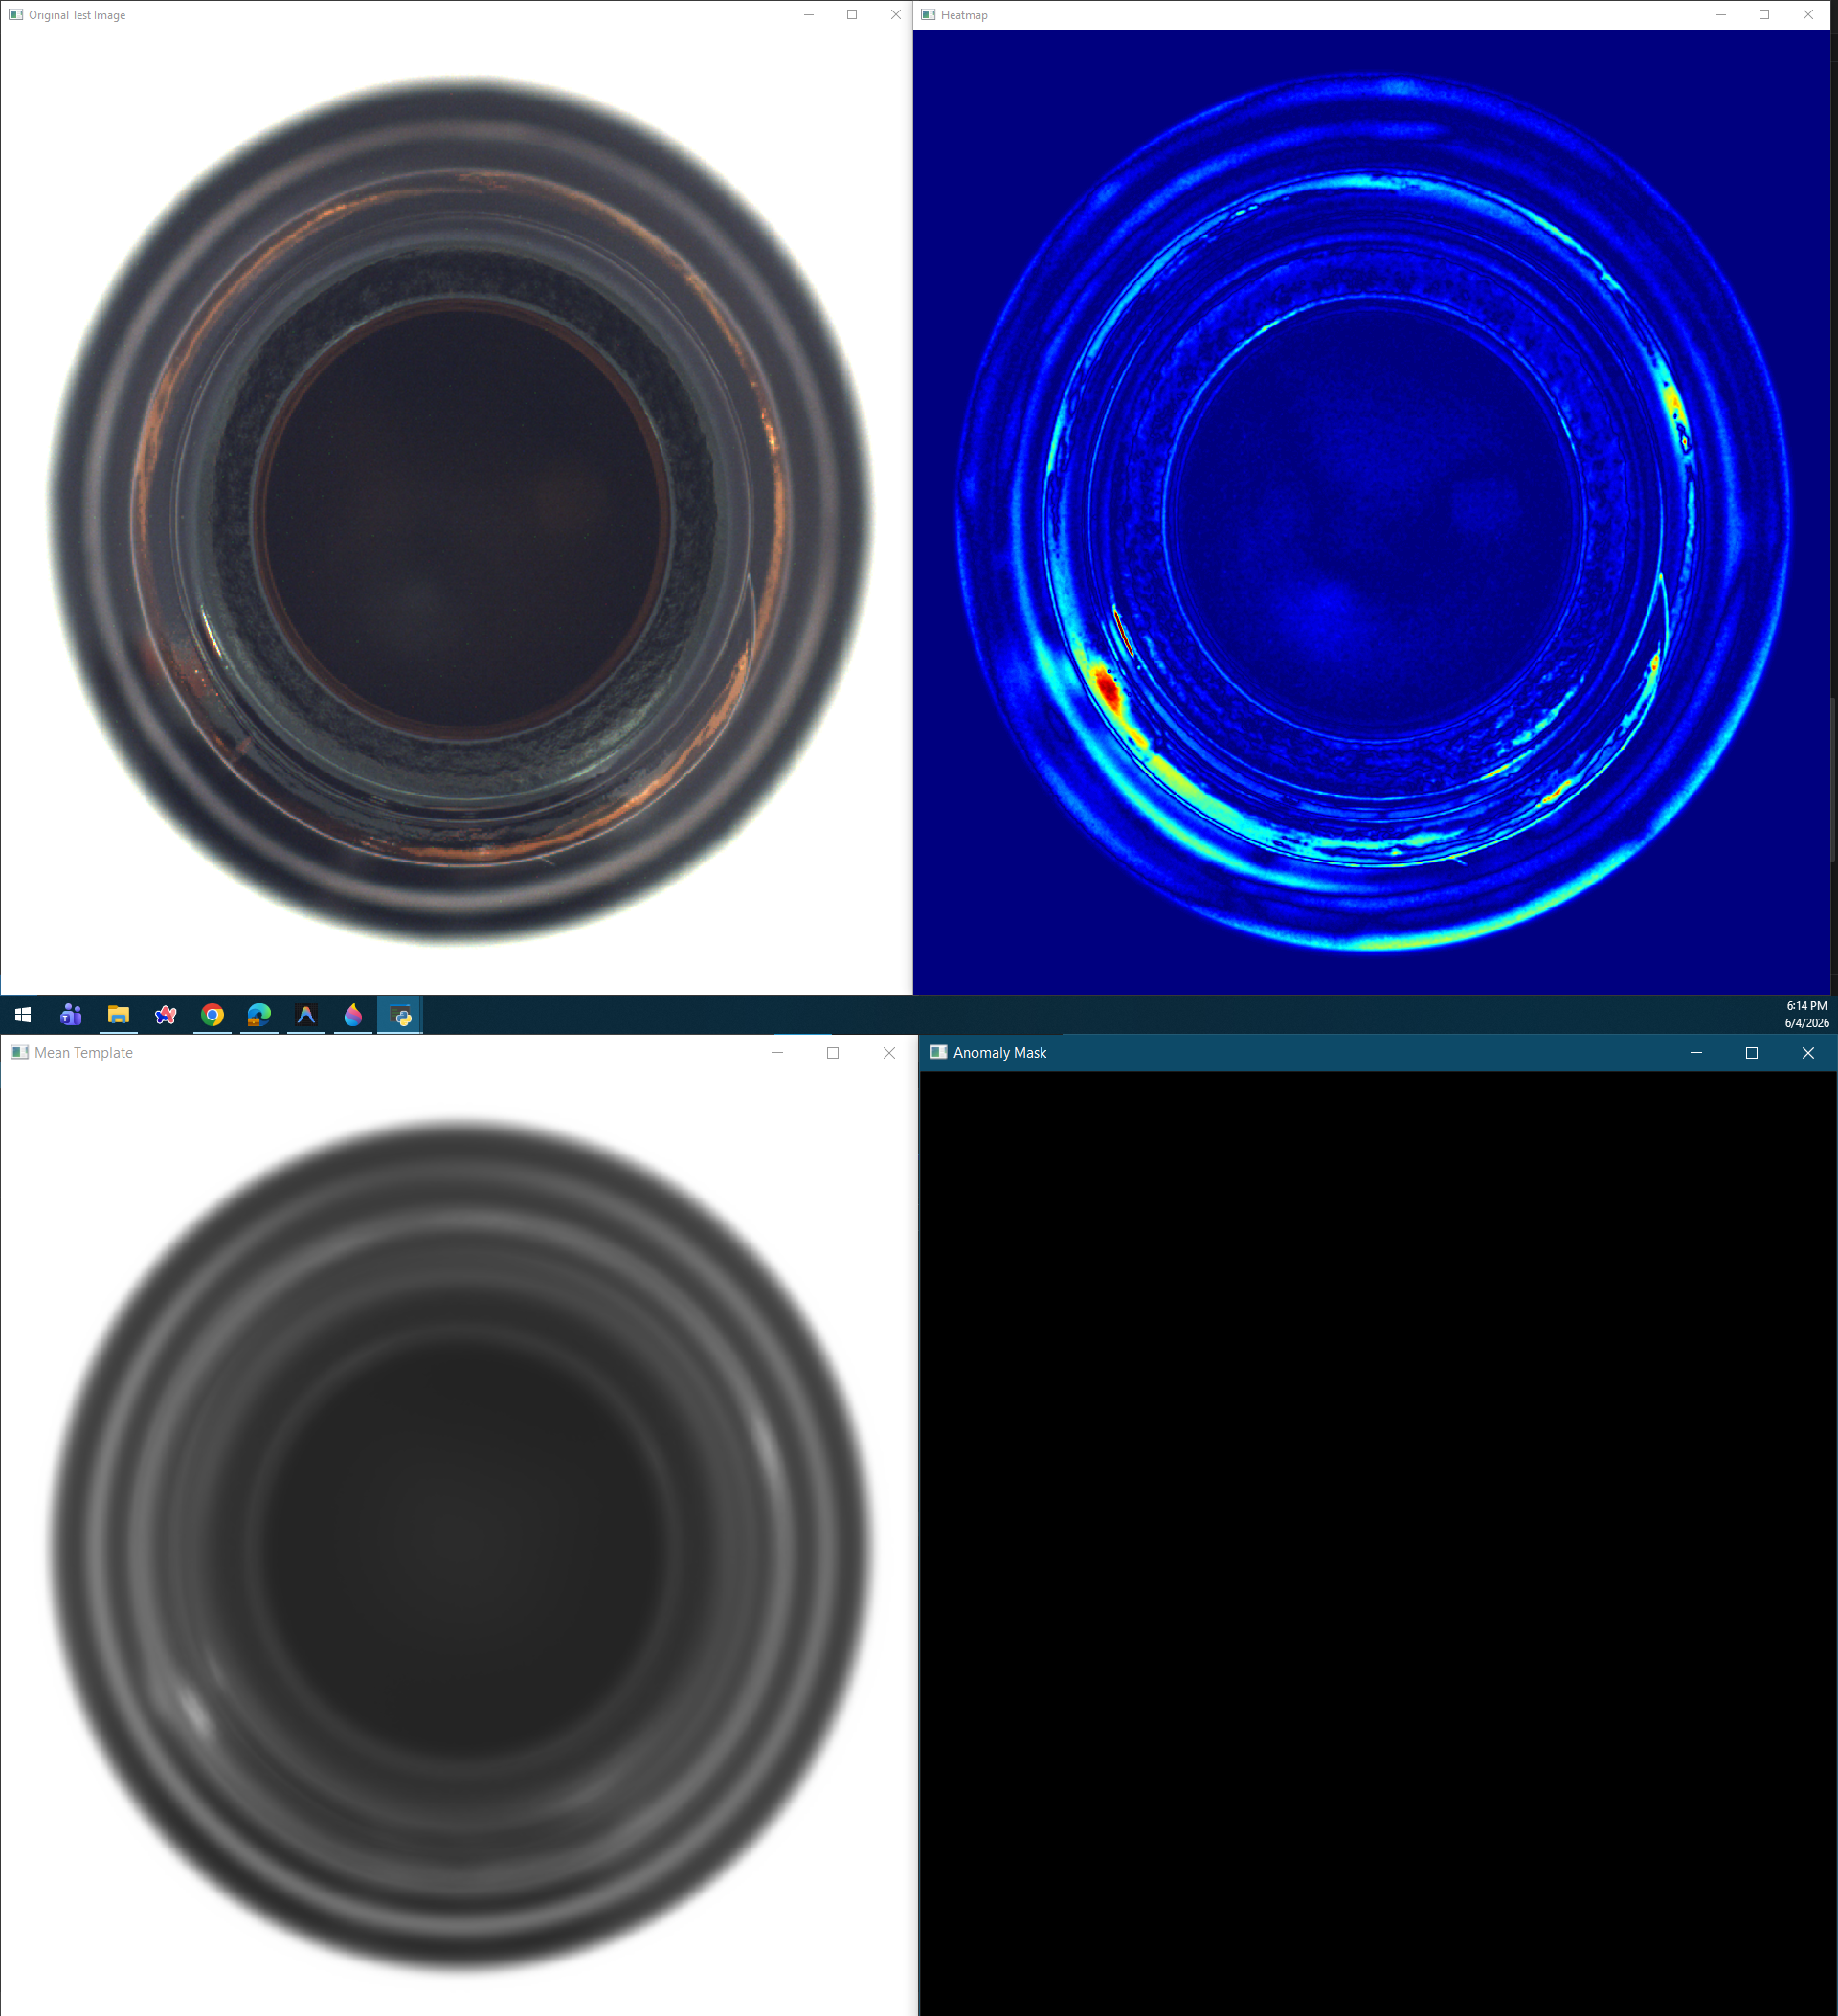
\includegraphics[width=0.8\textwidth]{runtime-images/bottle/bottle-good-result18.png}
    \caption{Bottle: bottle-good-result18.png}
\end{figure}

\subsection{Pill}
\begin{figure}[H]
    \centering
    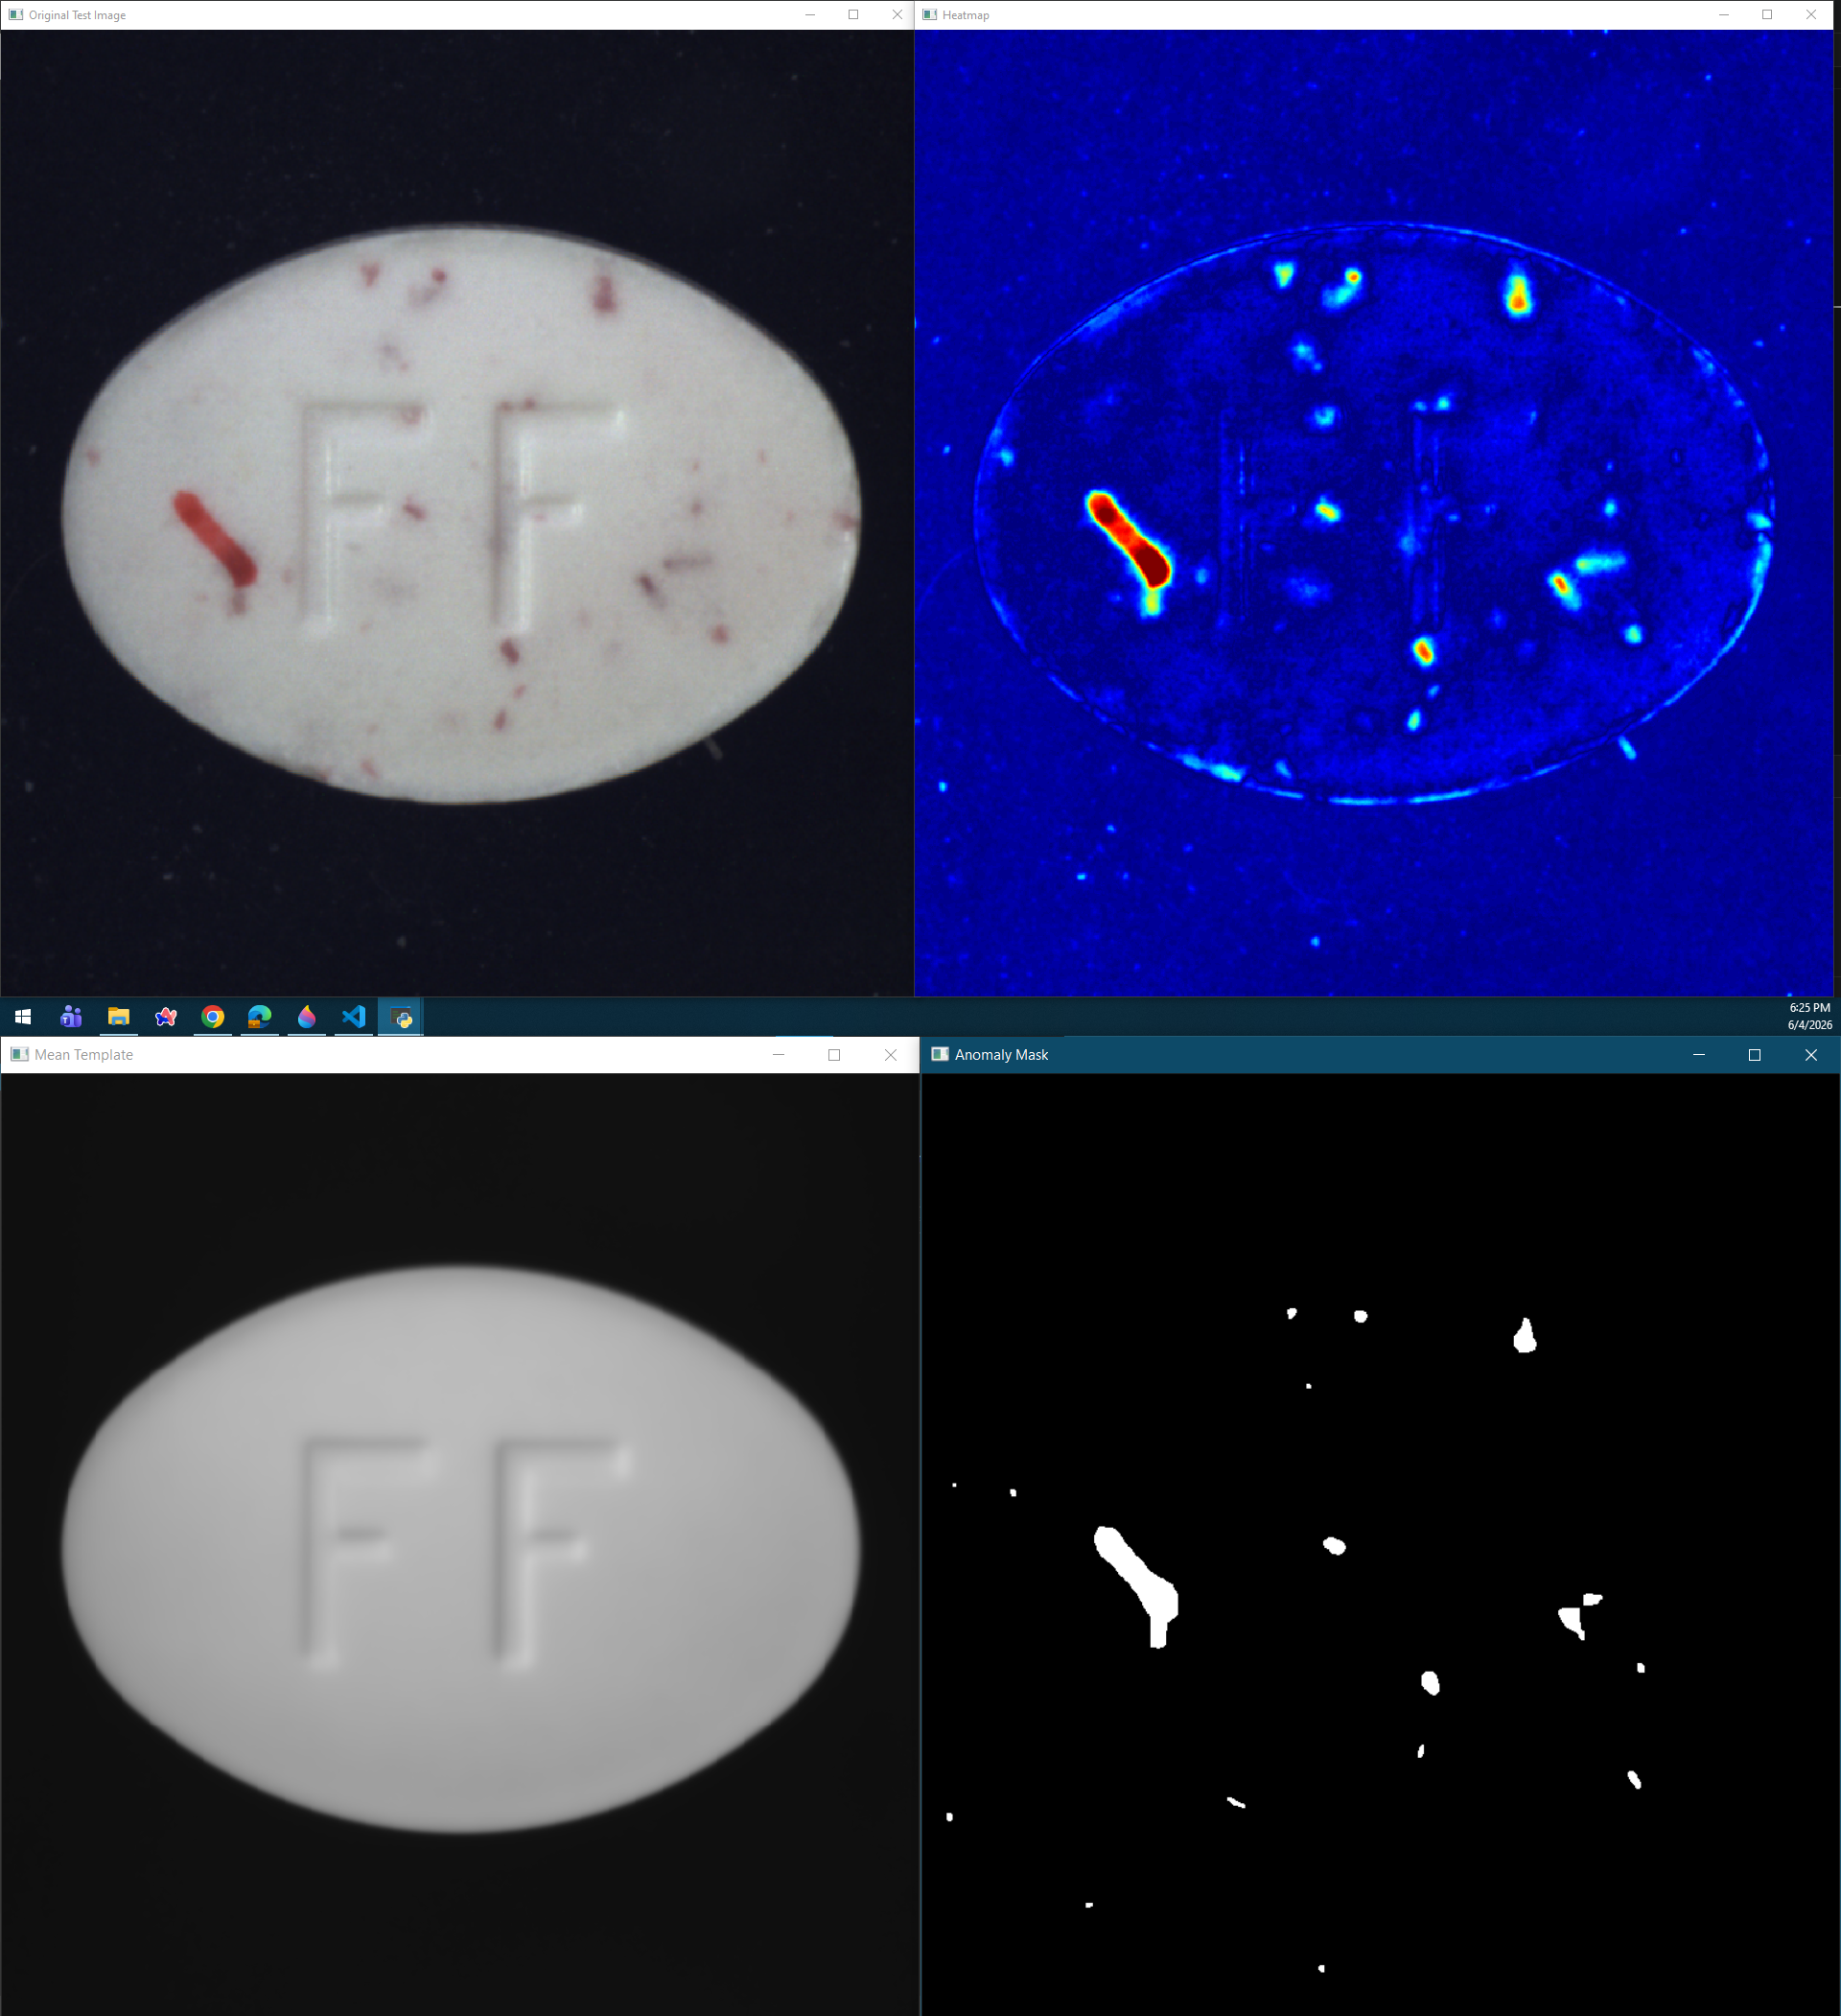
\includegraphics[width=0.8\textwidth]{runtime-images/pill/pill-color-result19.png}
    \caption{Pill: pill-color-result19.png}
\end{figure}

\begin{figure}[H]
    \centering
    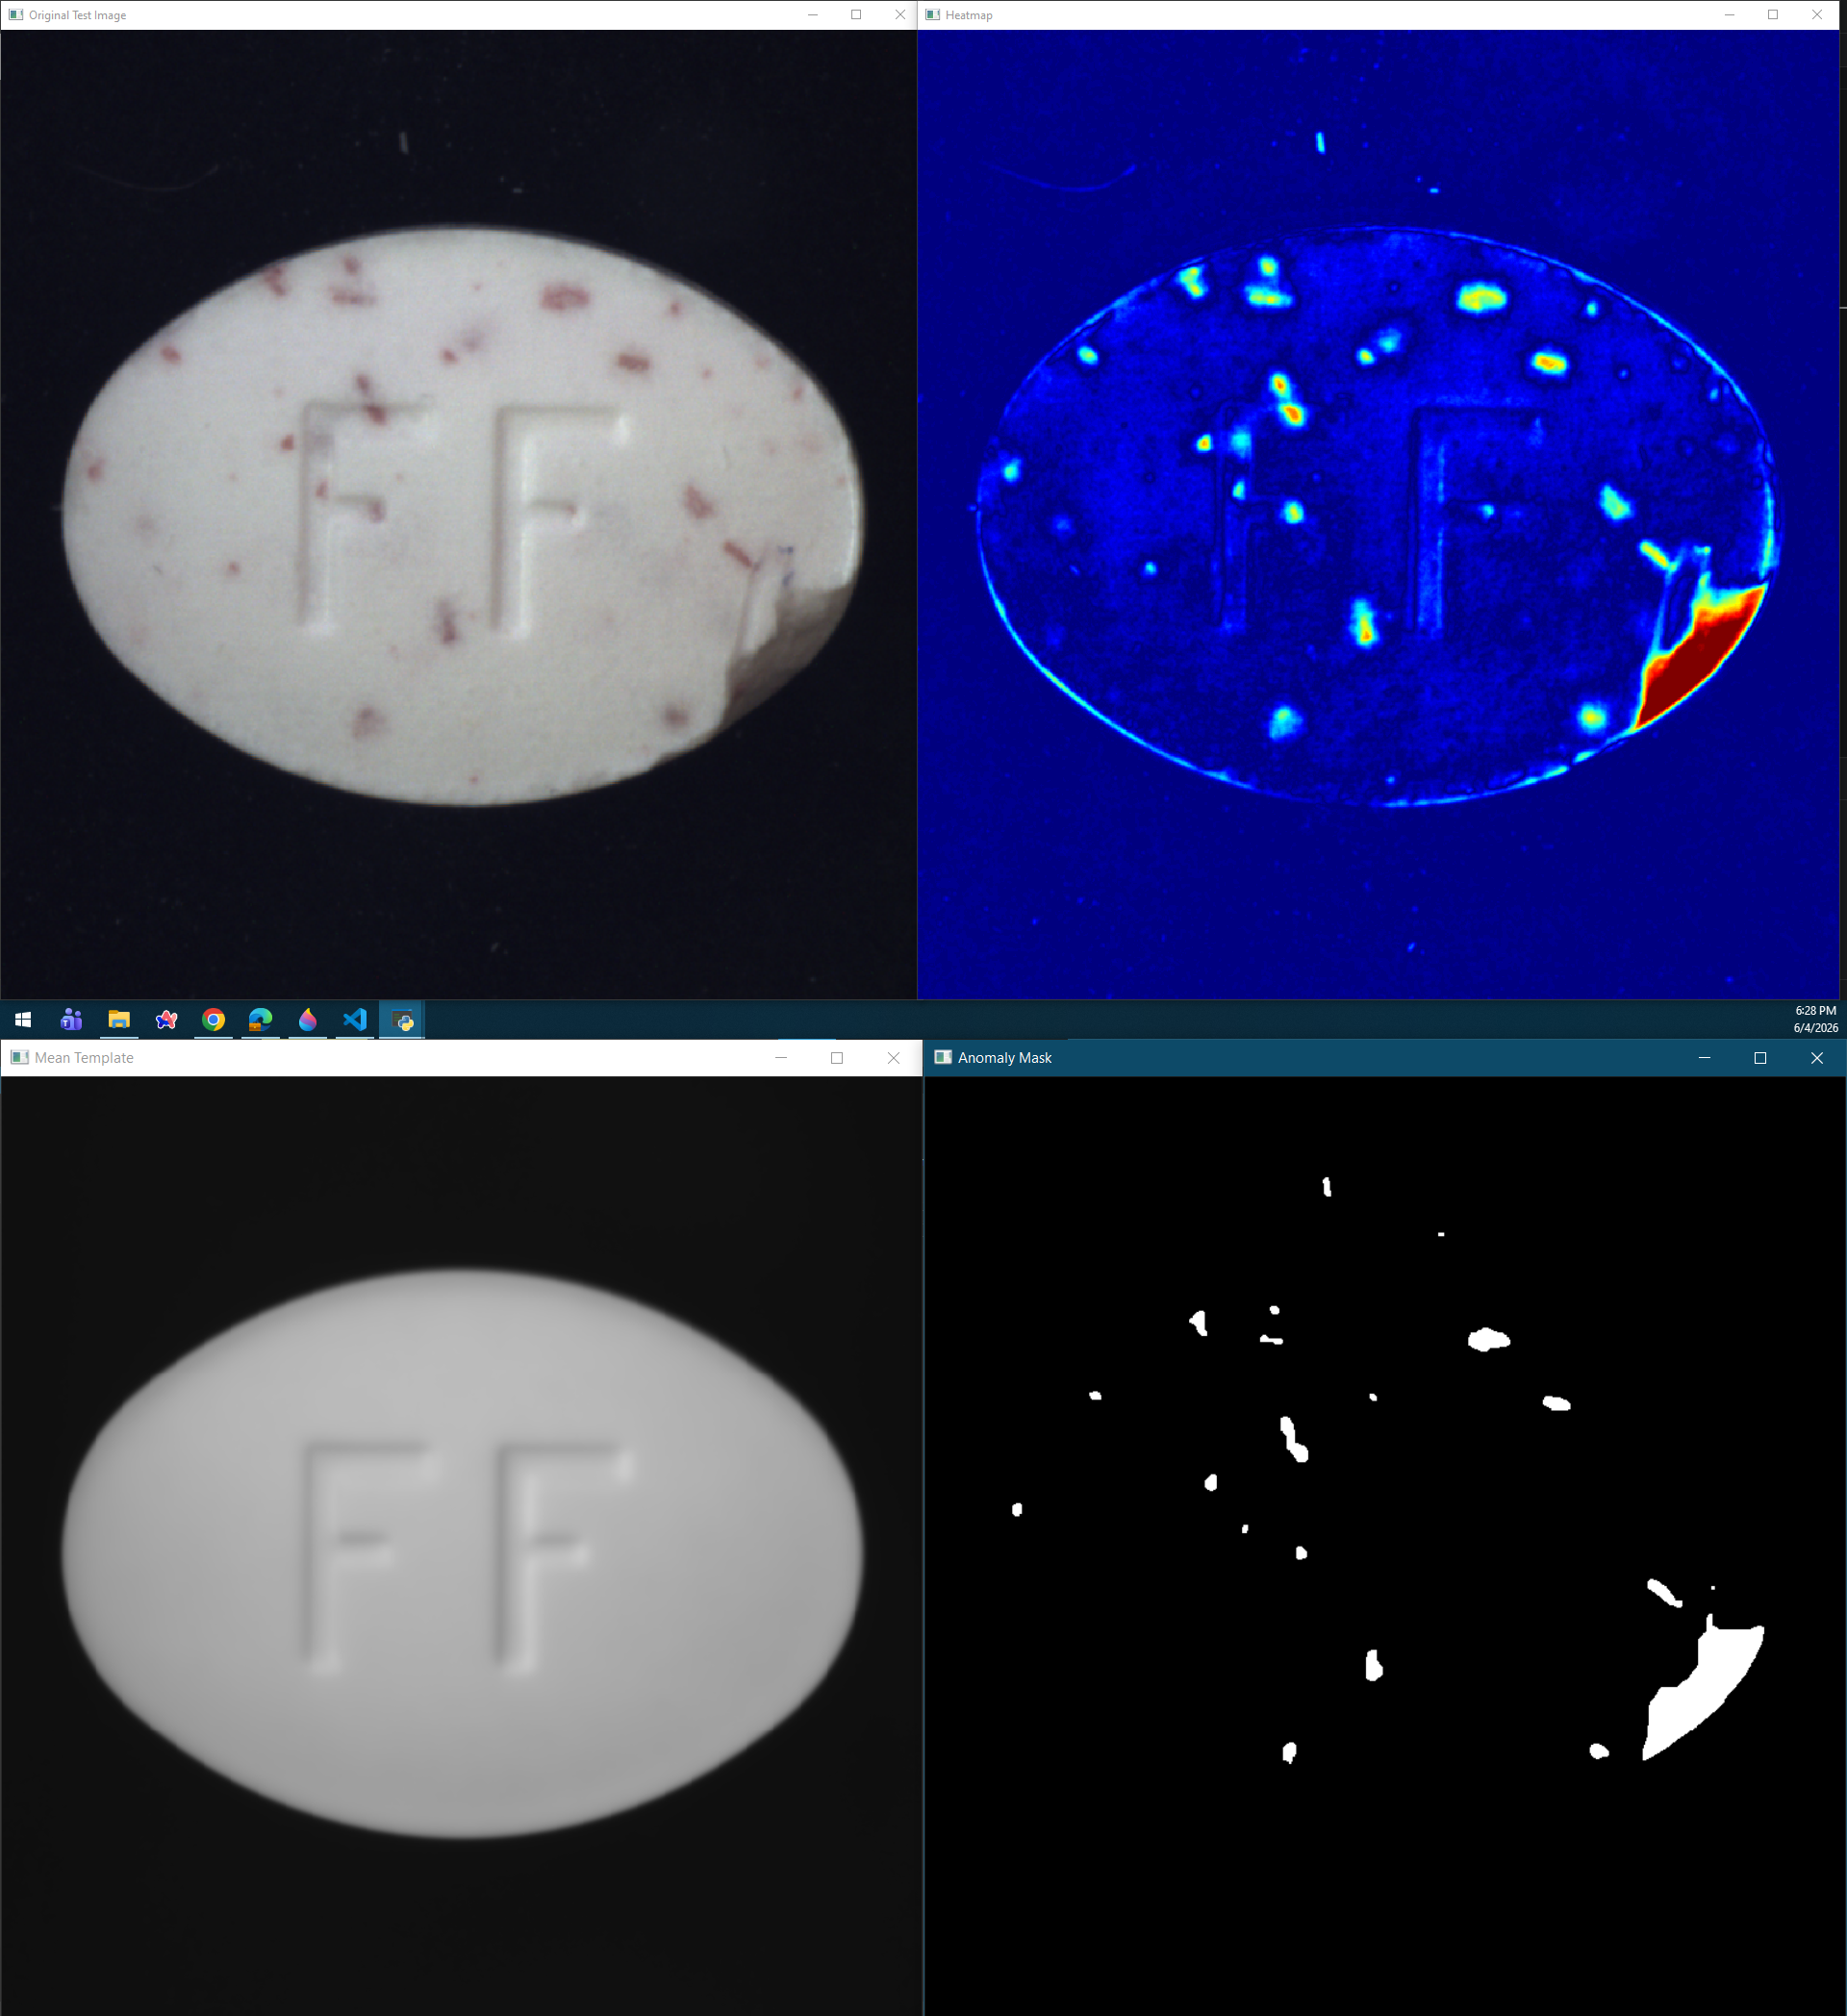
\includegraphics[width=0.8\textwidth]{runtime-images/pill/pill-crack-result5.png}
    \caption{Pill: pill-crack-result5.png}
\end{figure}

\begin{figure}[H]
    \centering
    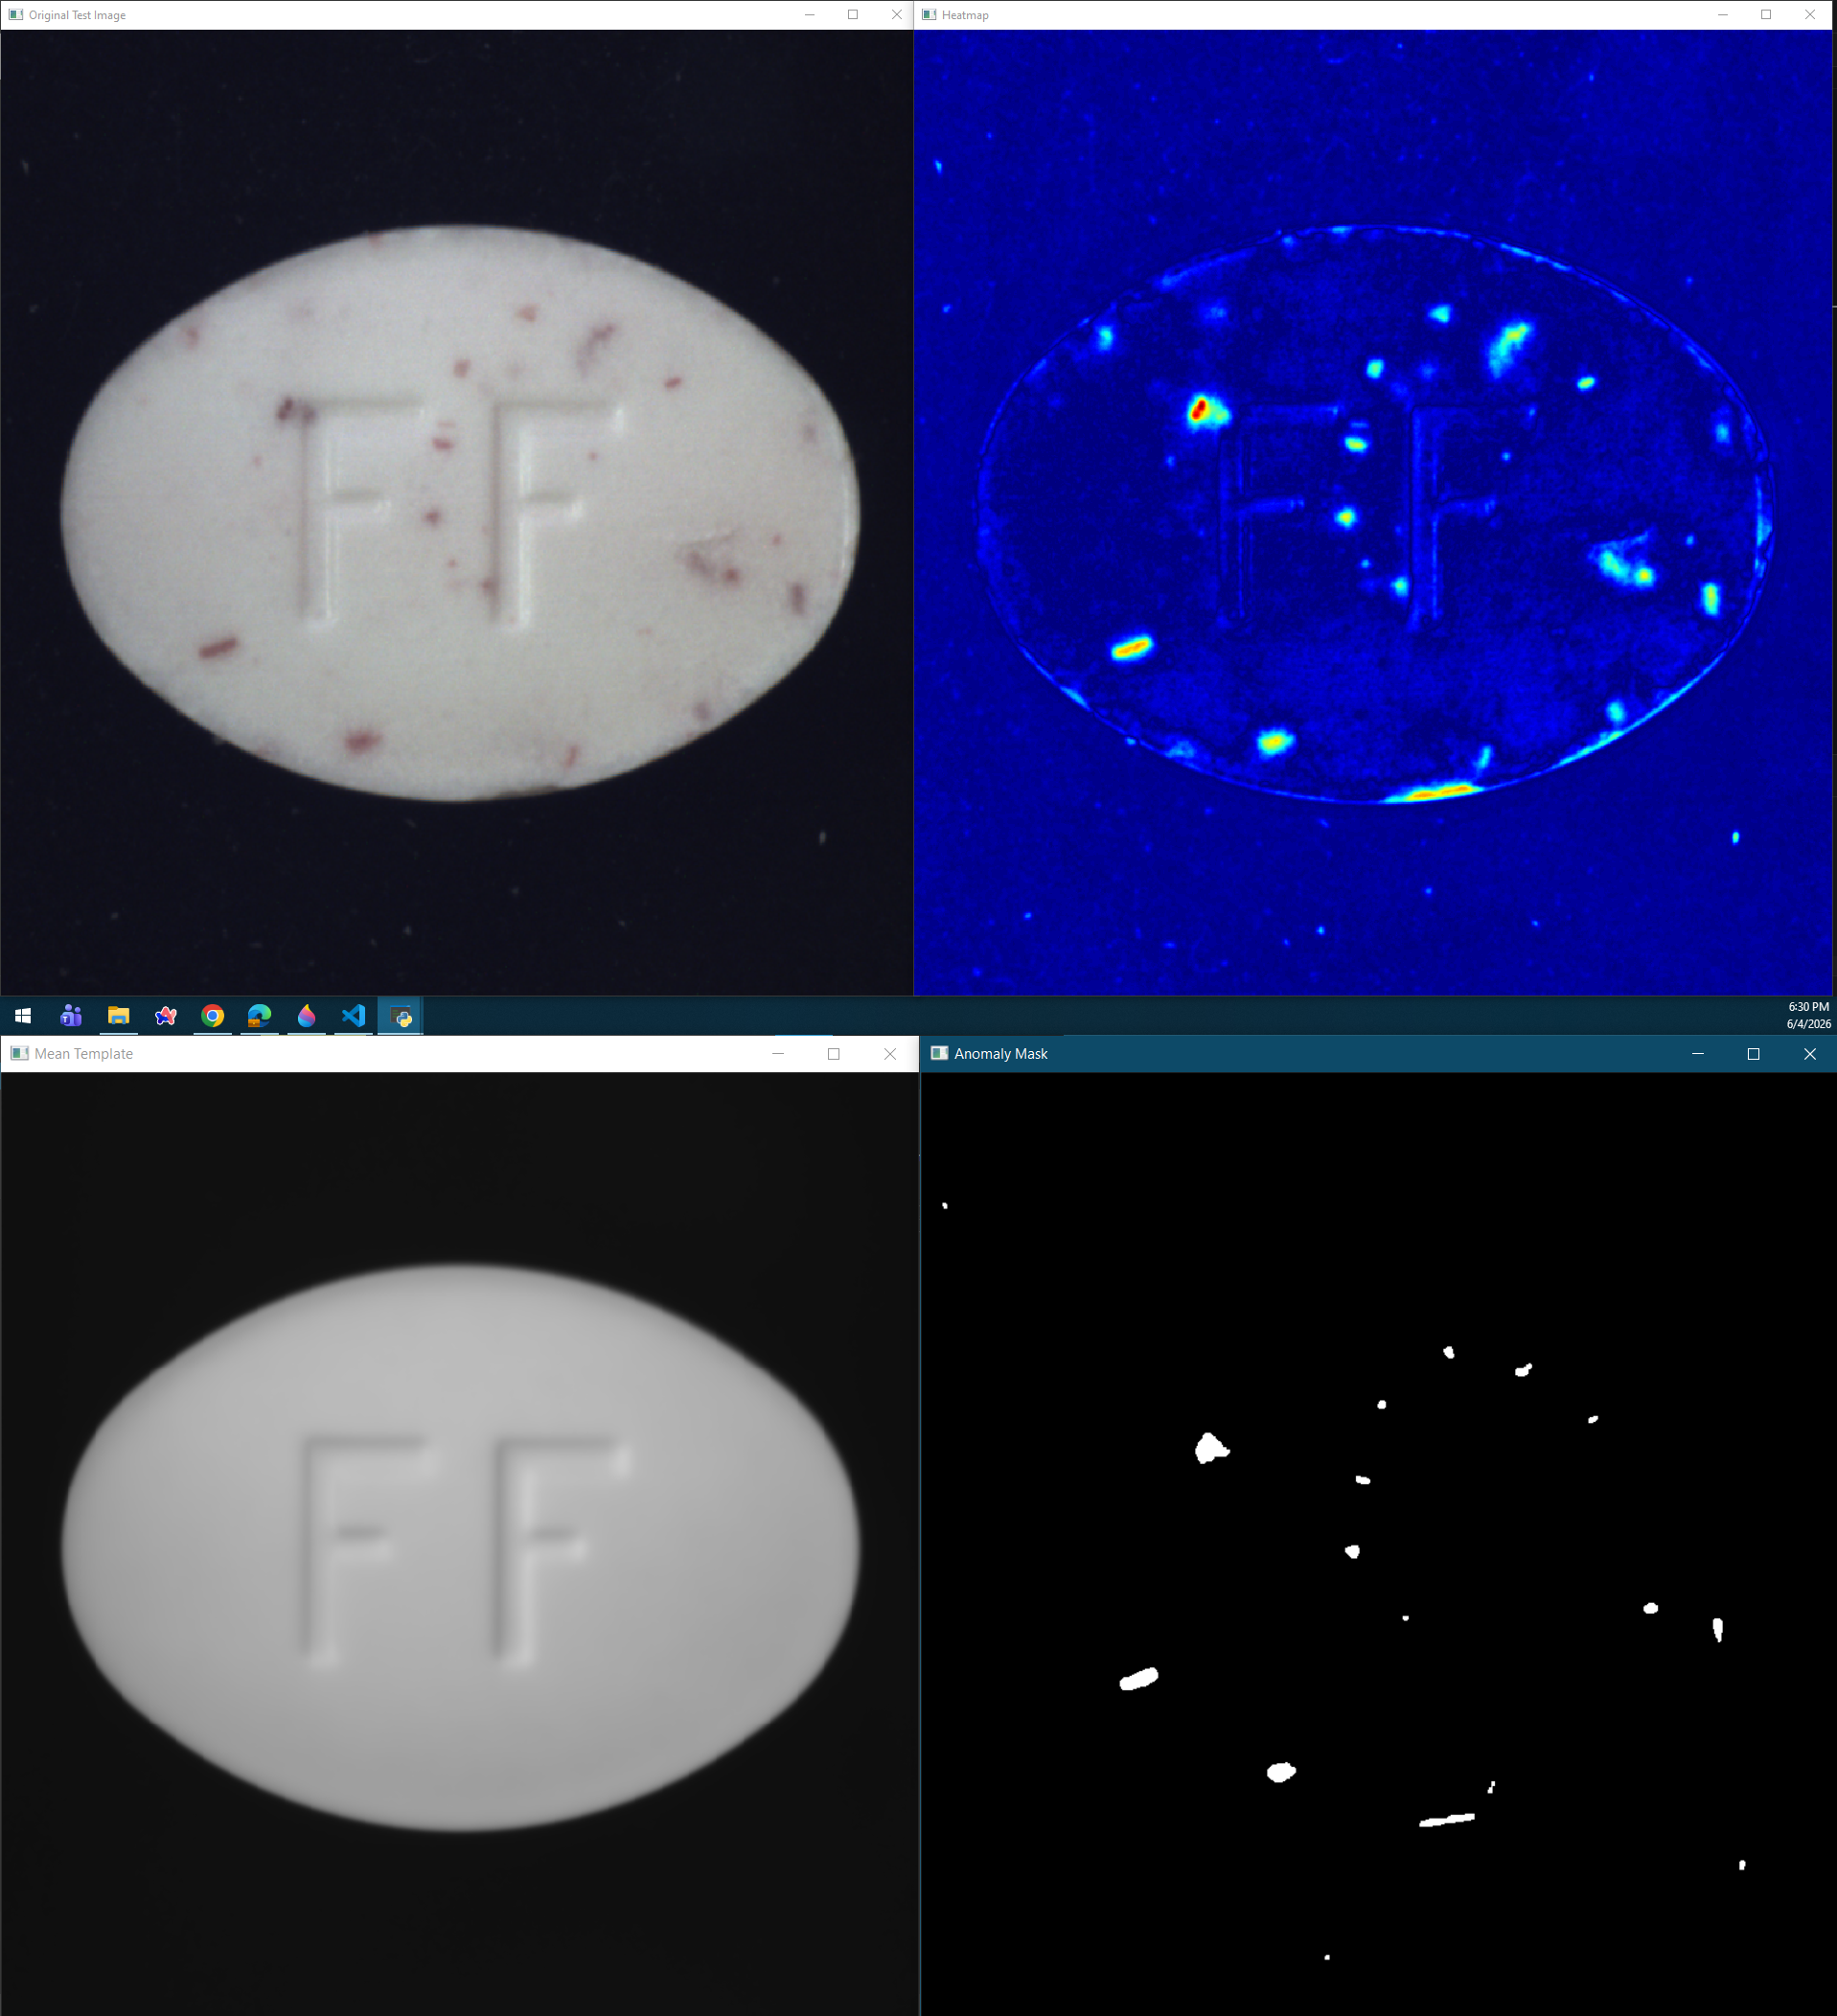
\includegraphics[width=0.8\textwidth]{runtime-images/pill/pill-good-result2.png}
    \caption{Pill: pill-good-result2.png}
\end{figure}

\begin{figure}[H]
    \centering
    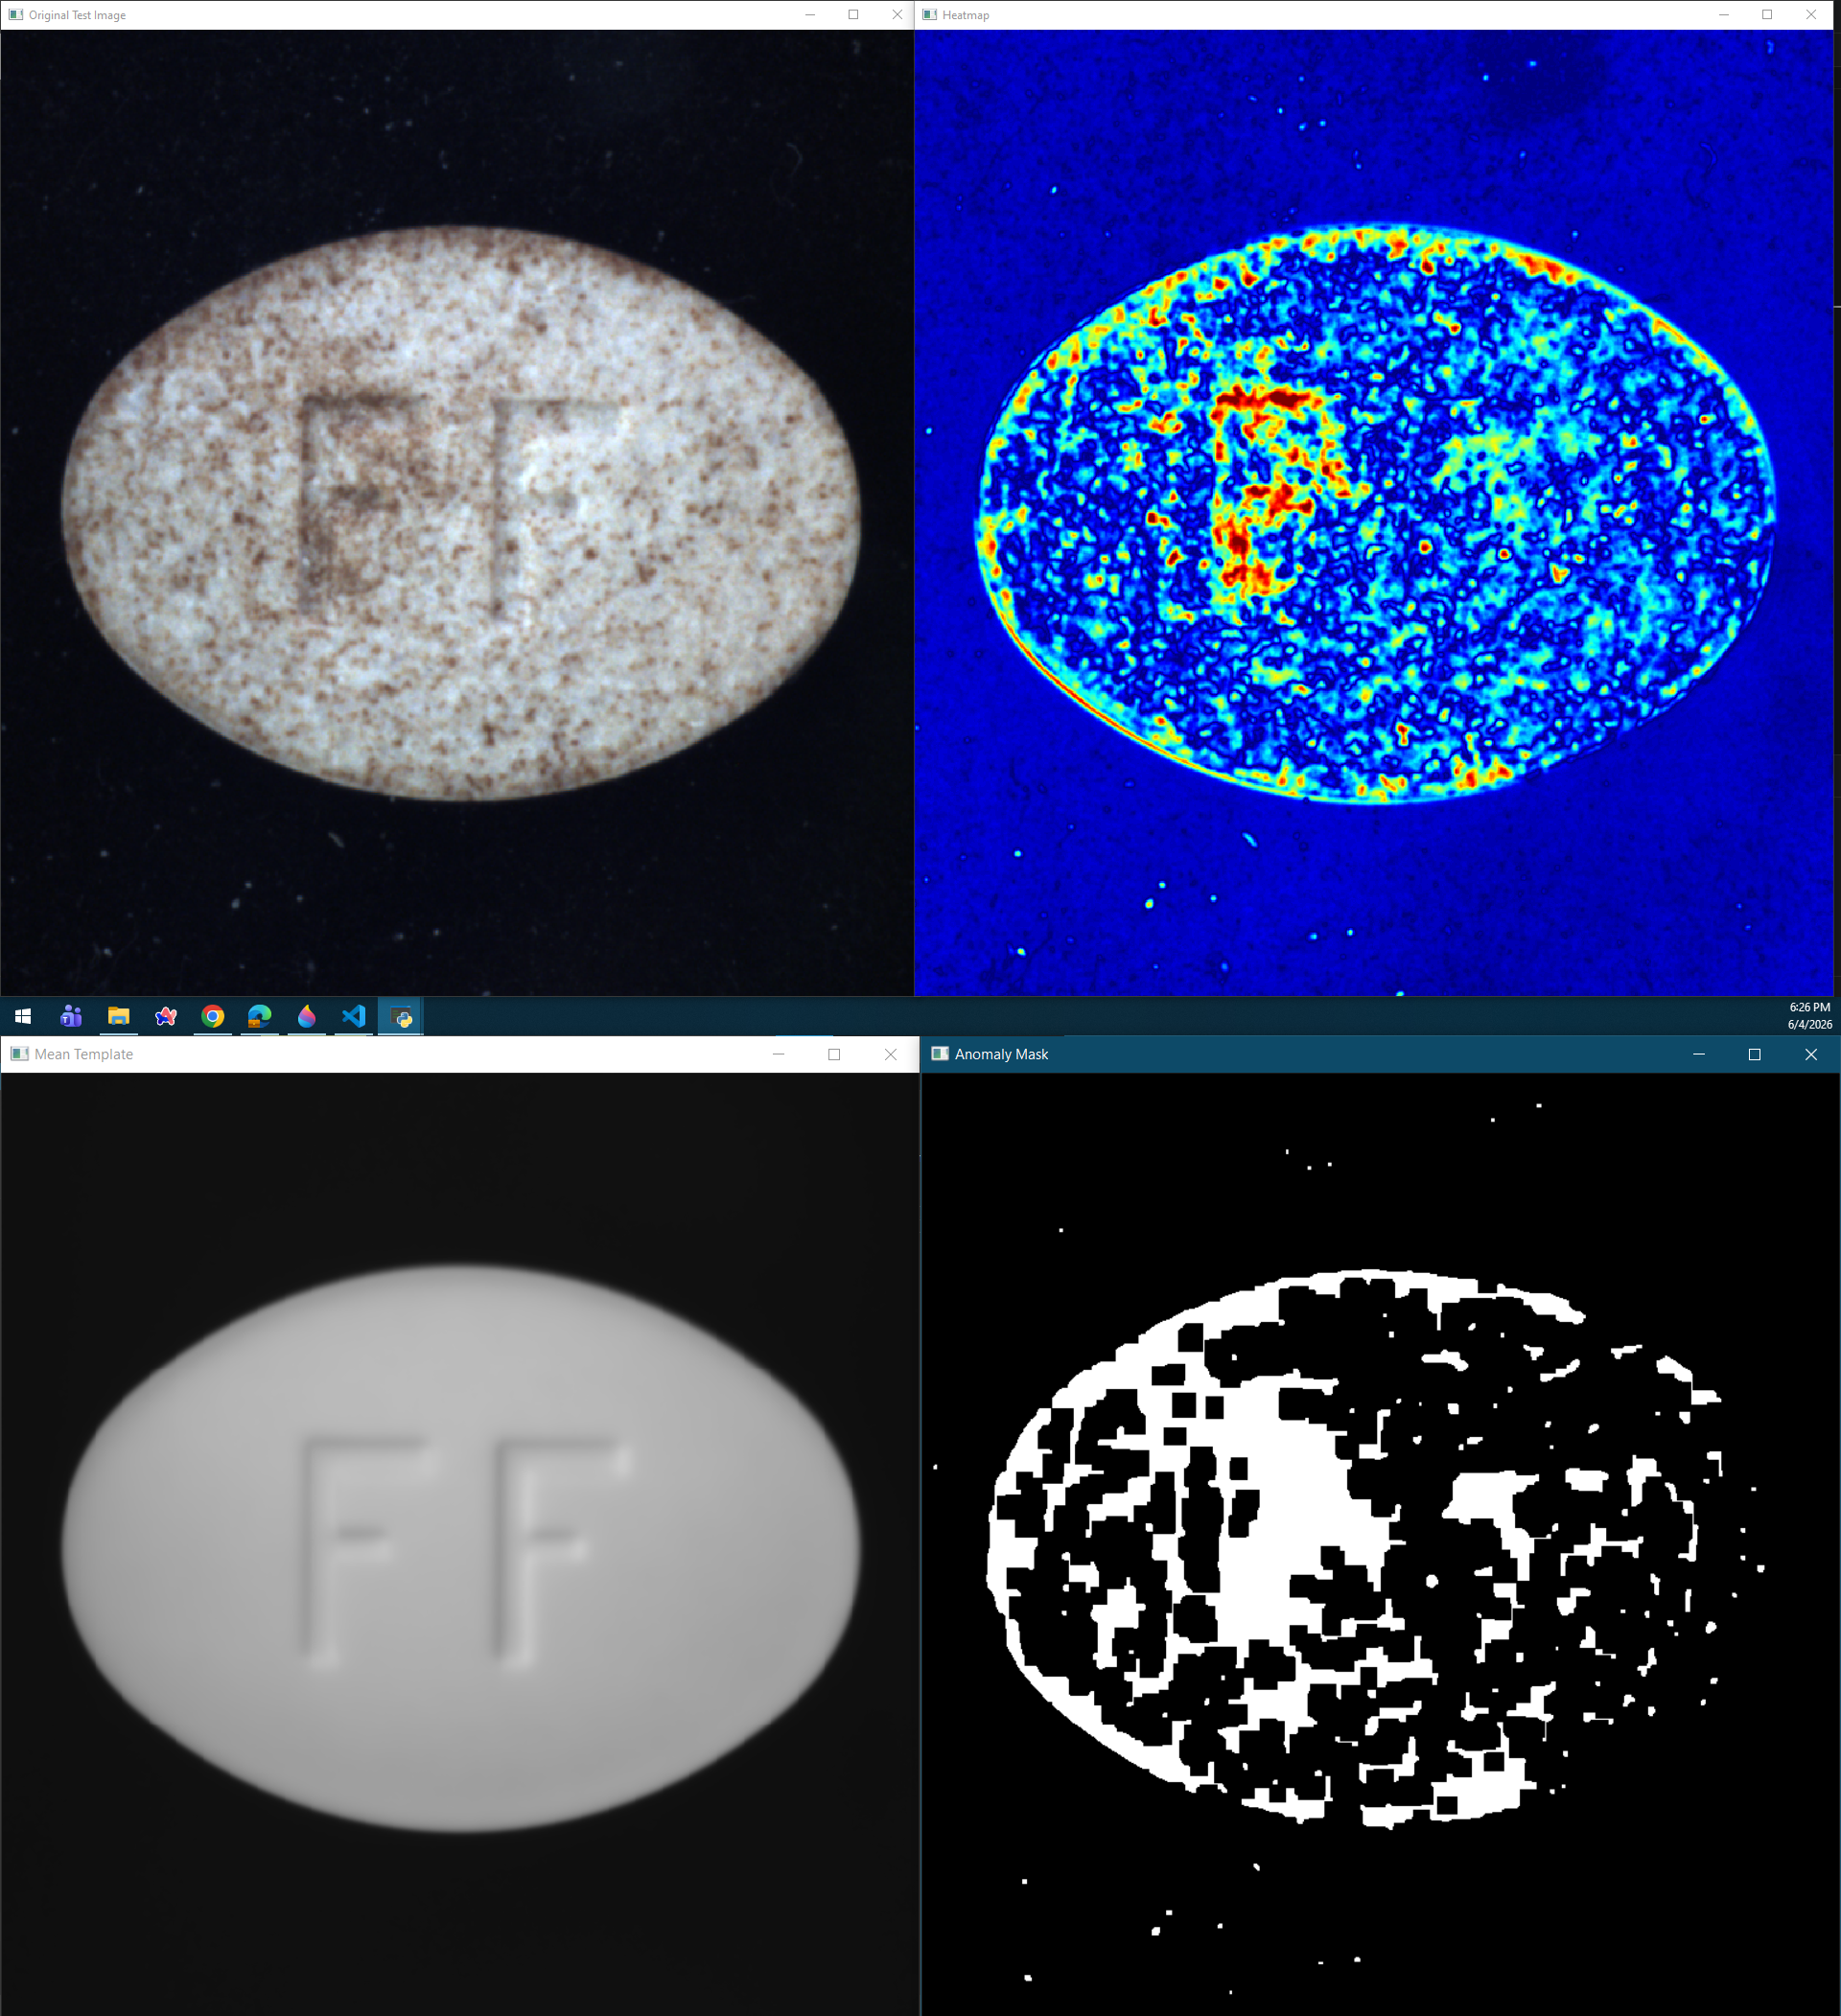
\includegraphics[width=0.8\textwidth]{runtime-images/pill/pill-pill_type-result0.png}
    \caption{Pill: pill-pill\_type-result0.png}
\end{figure}

\subsection{Wood}
\begin{figure}[H]
    \centering
    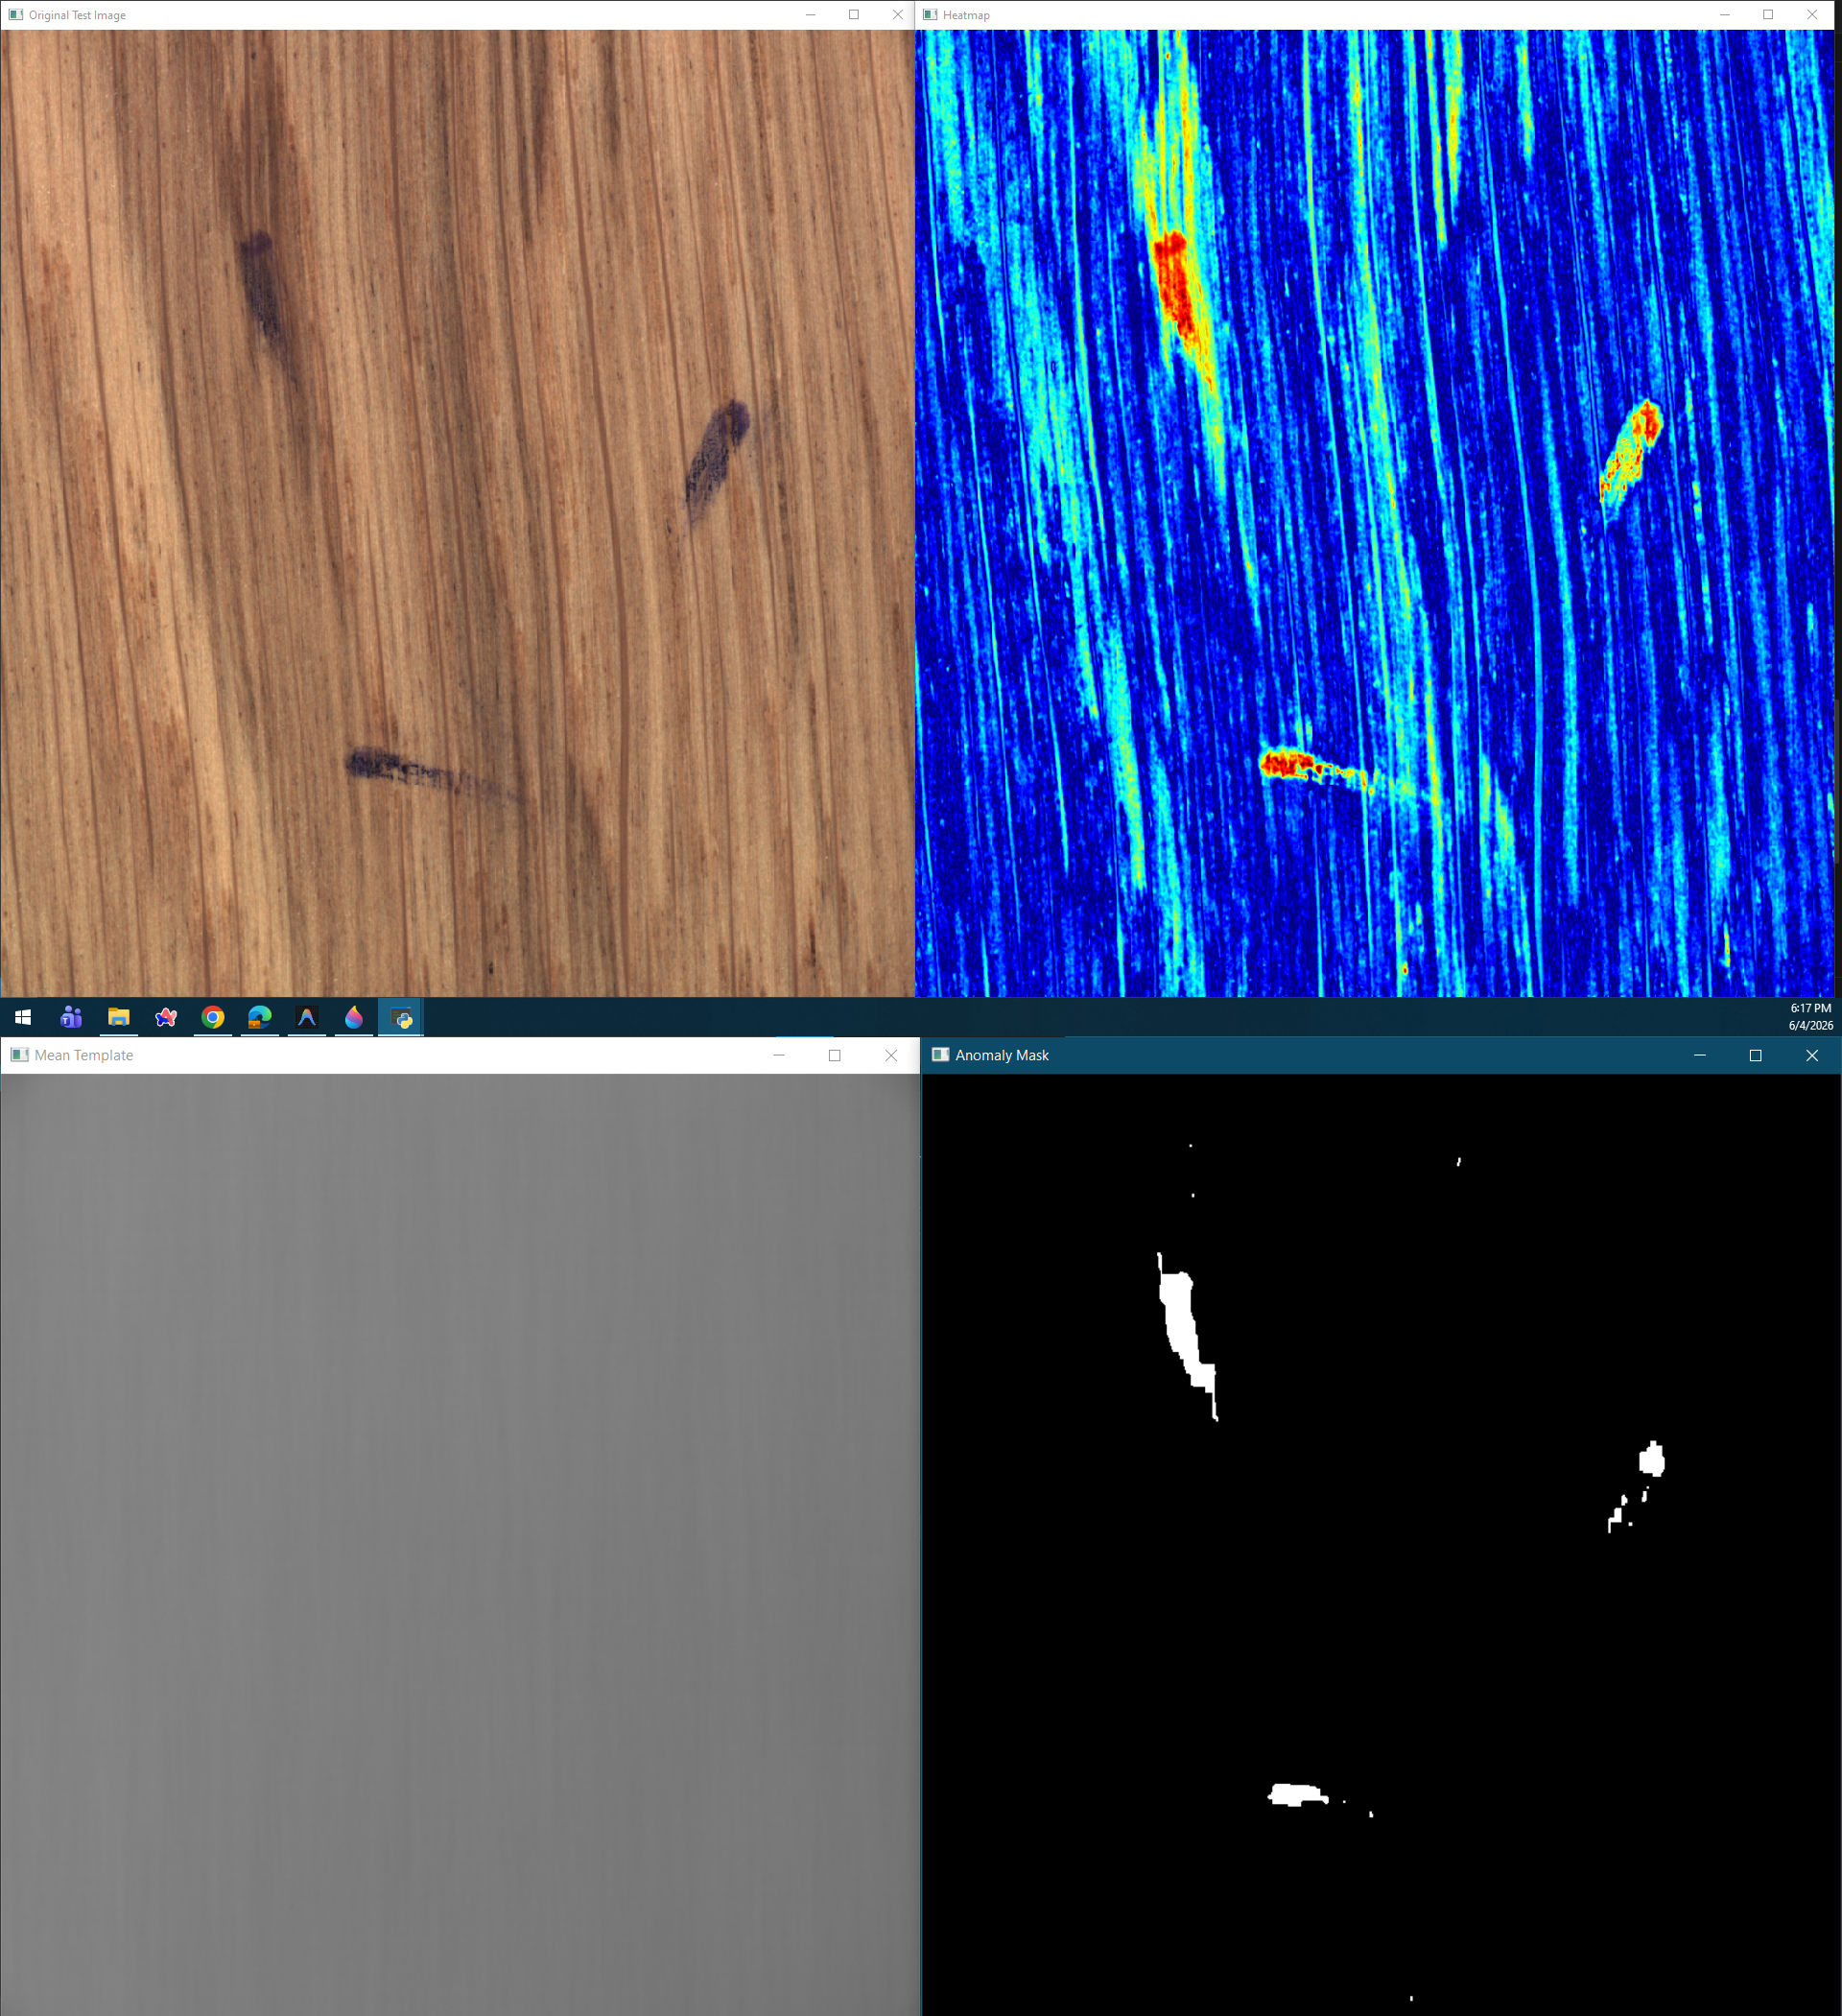
\includegraphics[width=0.8\textwidth]{runtime-images/wood/wood-color-result5.png}
    \caption{Wood: wood-color-result5.png}
\end{figure}

\begin{figure}[H]
    \centering
    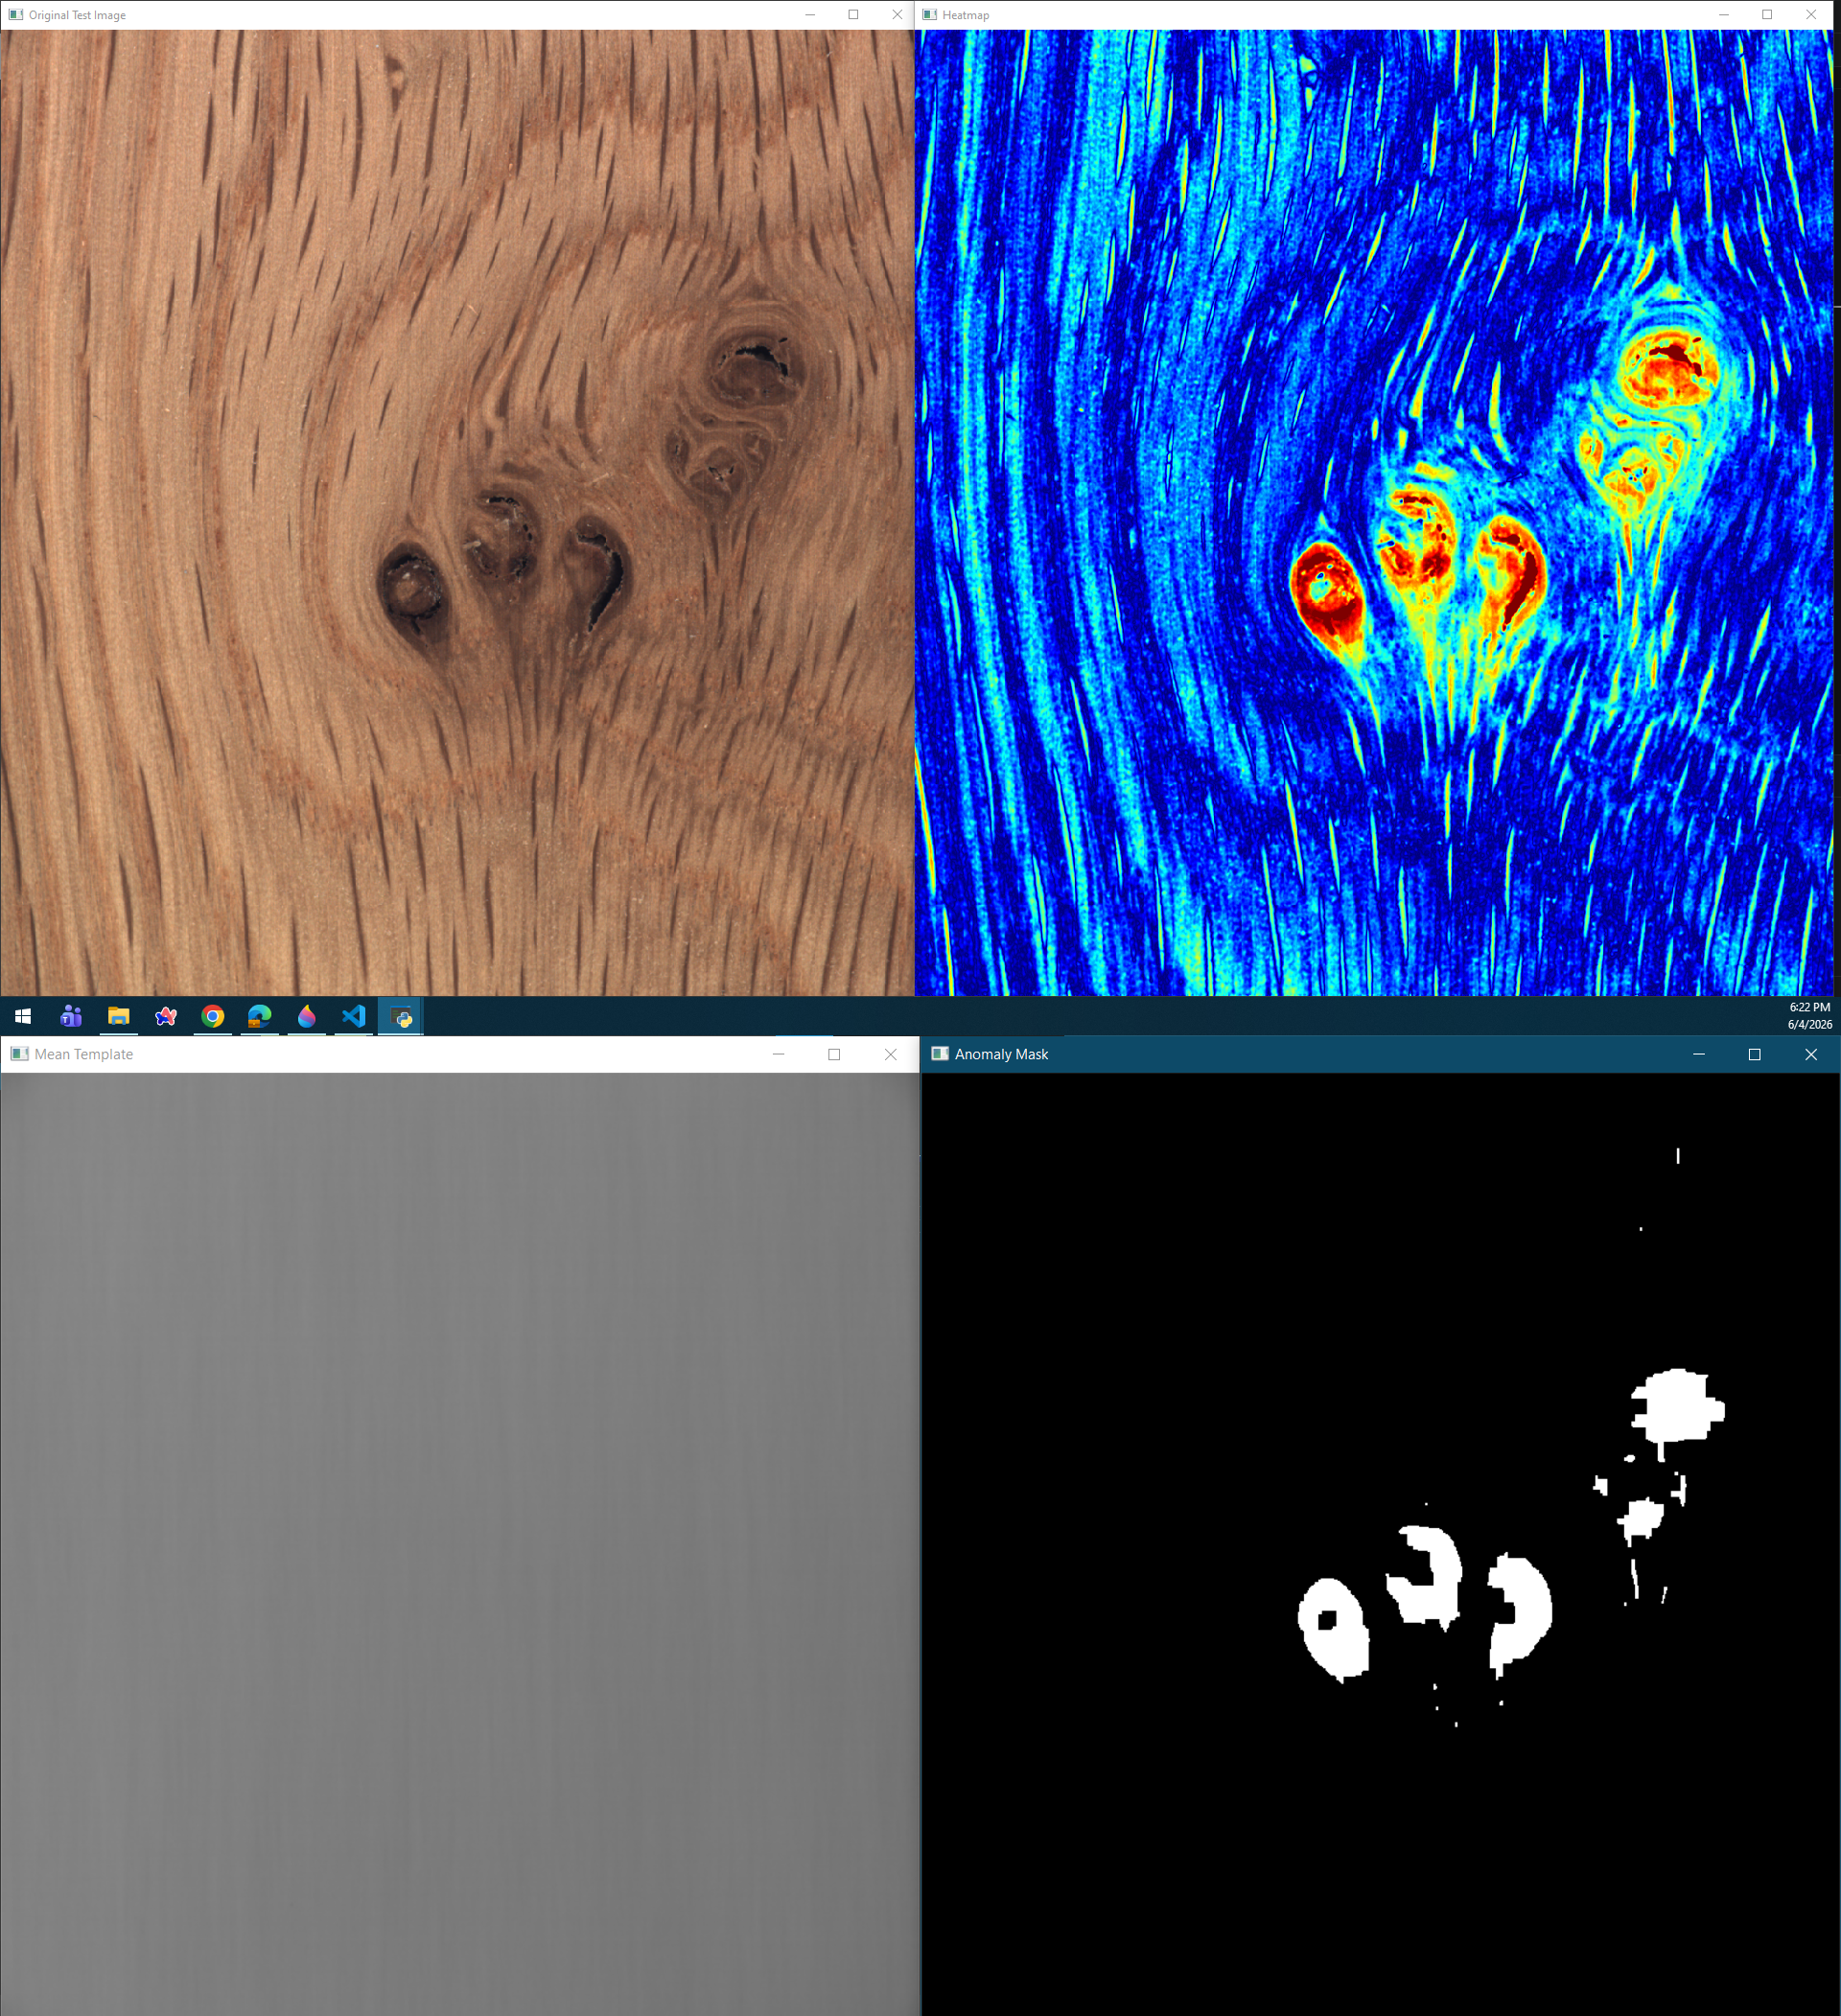
\includegraphics[width=0.8\textwidth]{runtime-images/wood/wood-combined-result6.png}
    \caption{Wood: wood-combined-result6.png}
\end{figure}

\begin{figure}[H]
    \centering
    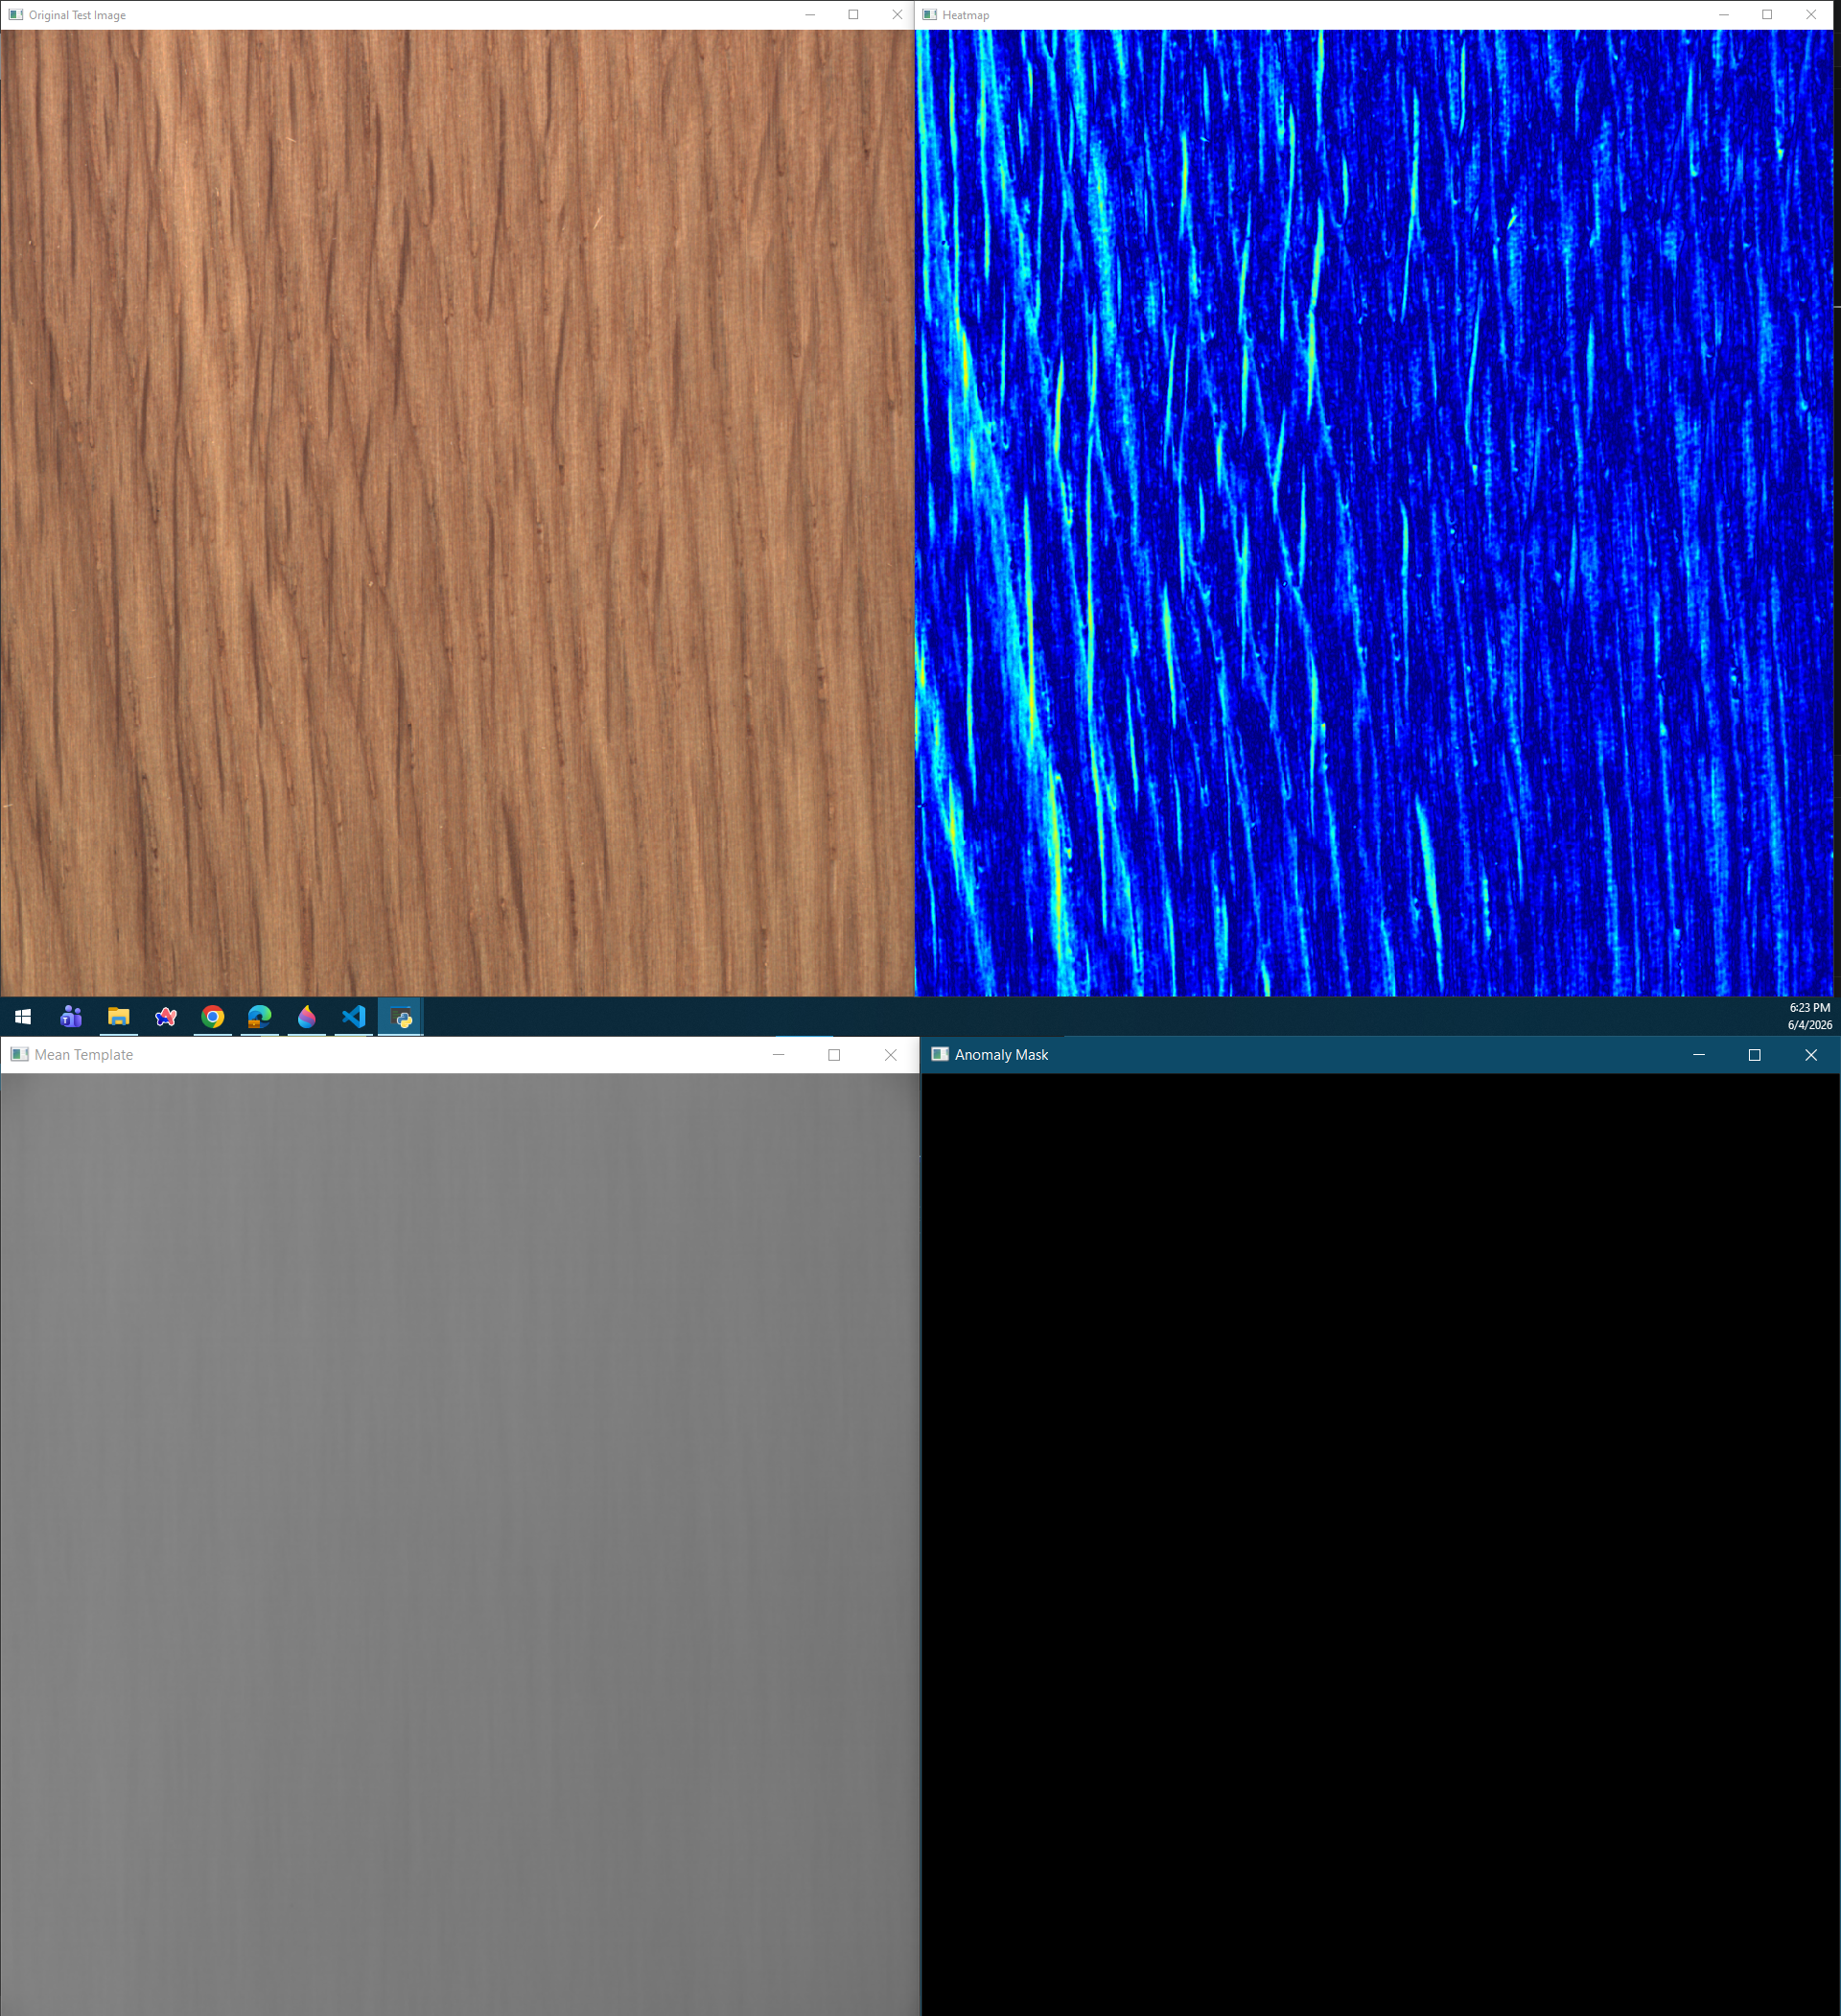
\includegraphics[width=0.8\textwidth]{runtime-images/wood/wood-good-result1.png}
    \caption{Wood: wood-good-result1.png}
\end{figure}

\begin{figure}[H]
    \centering
    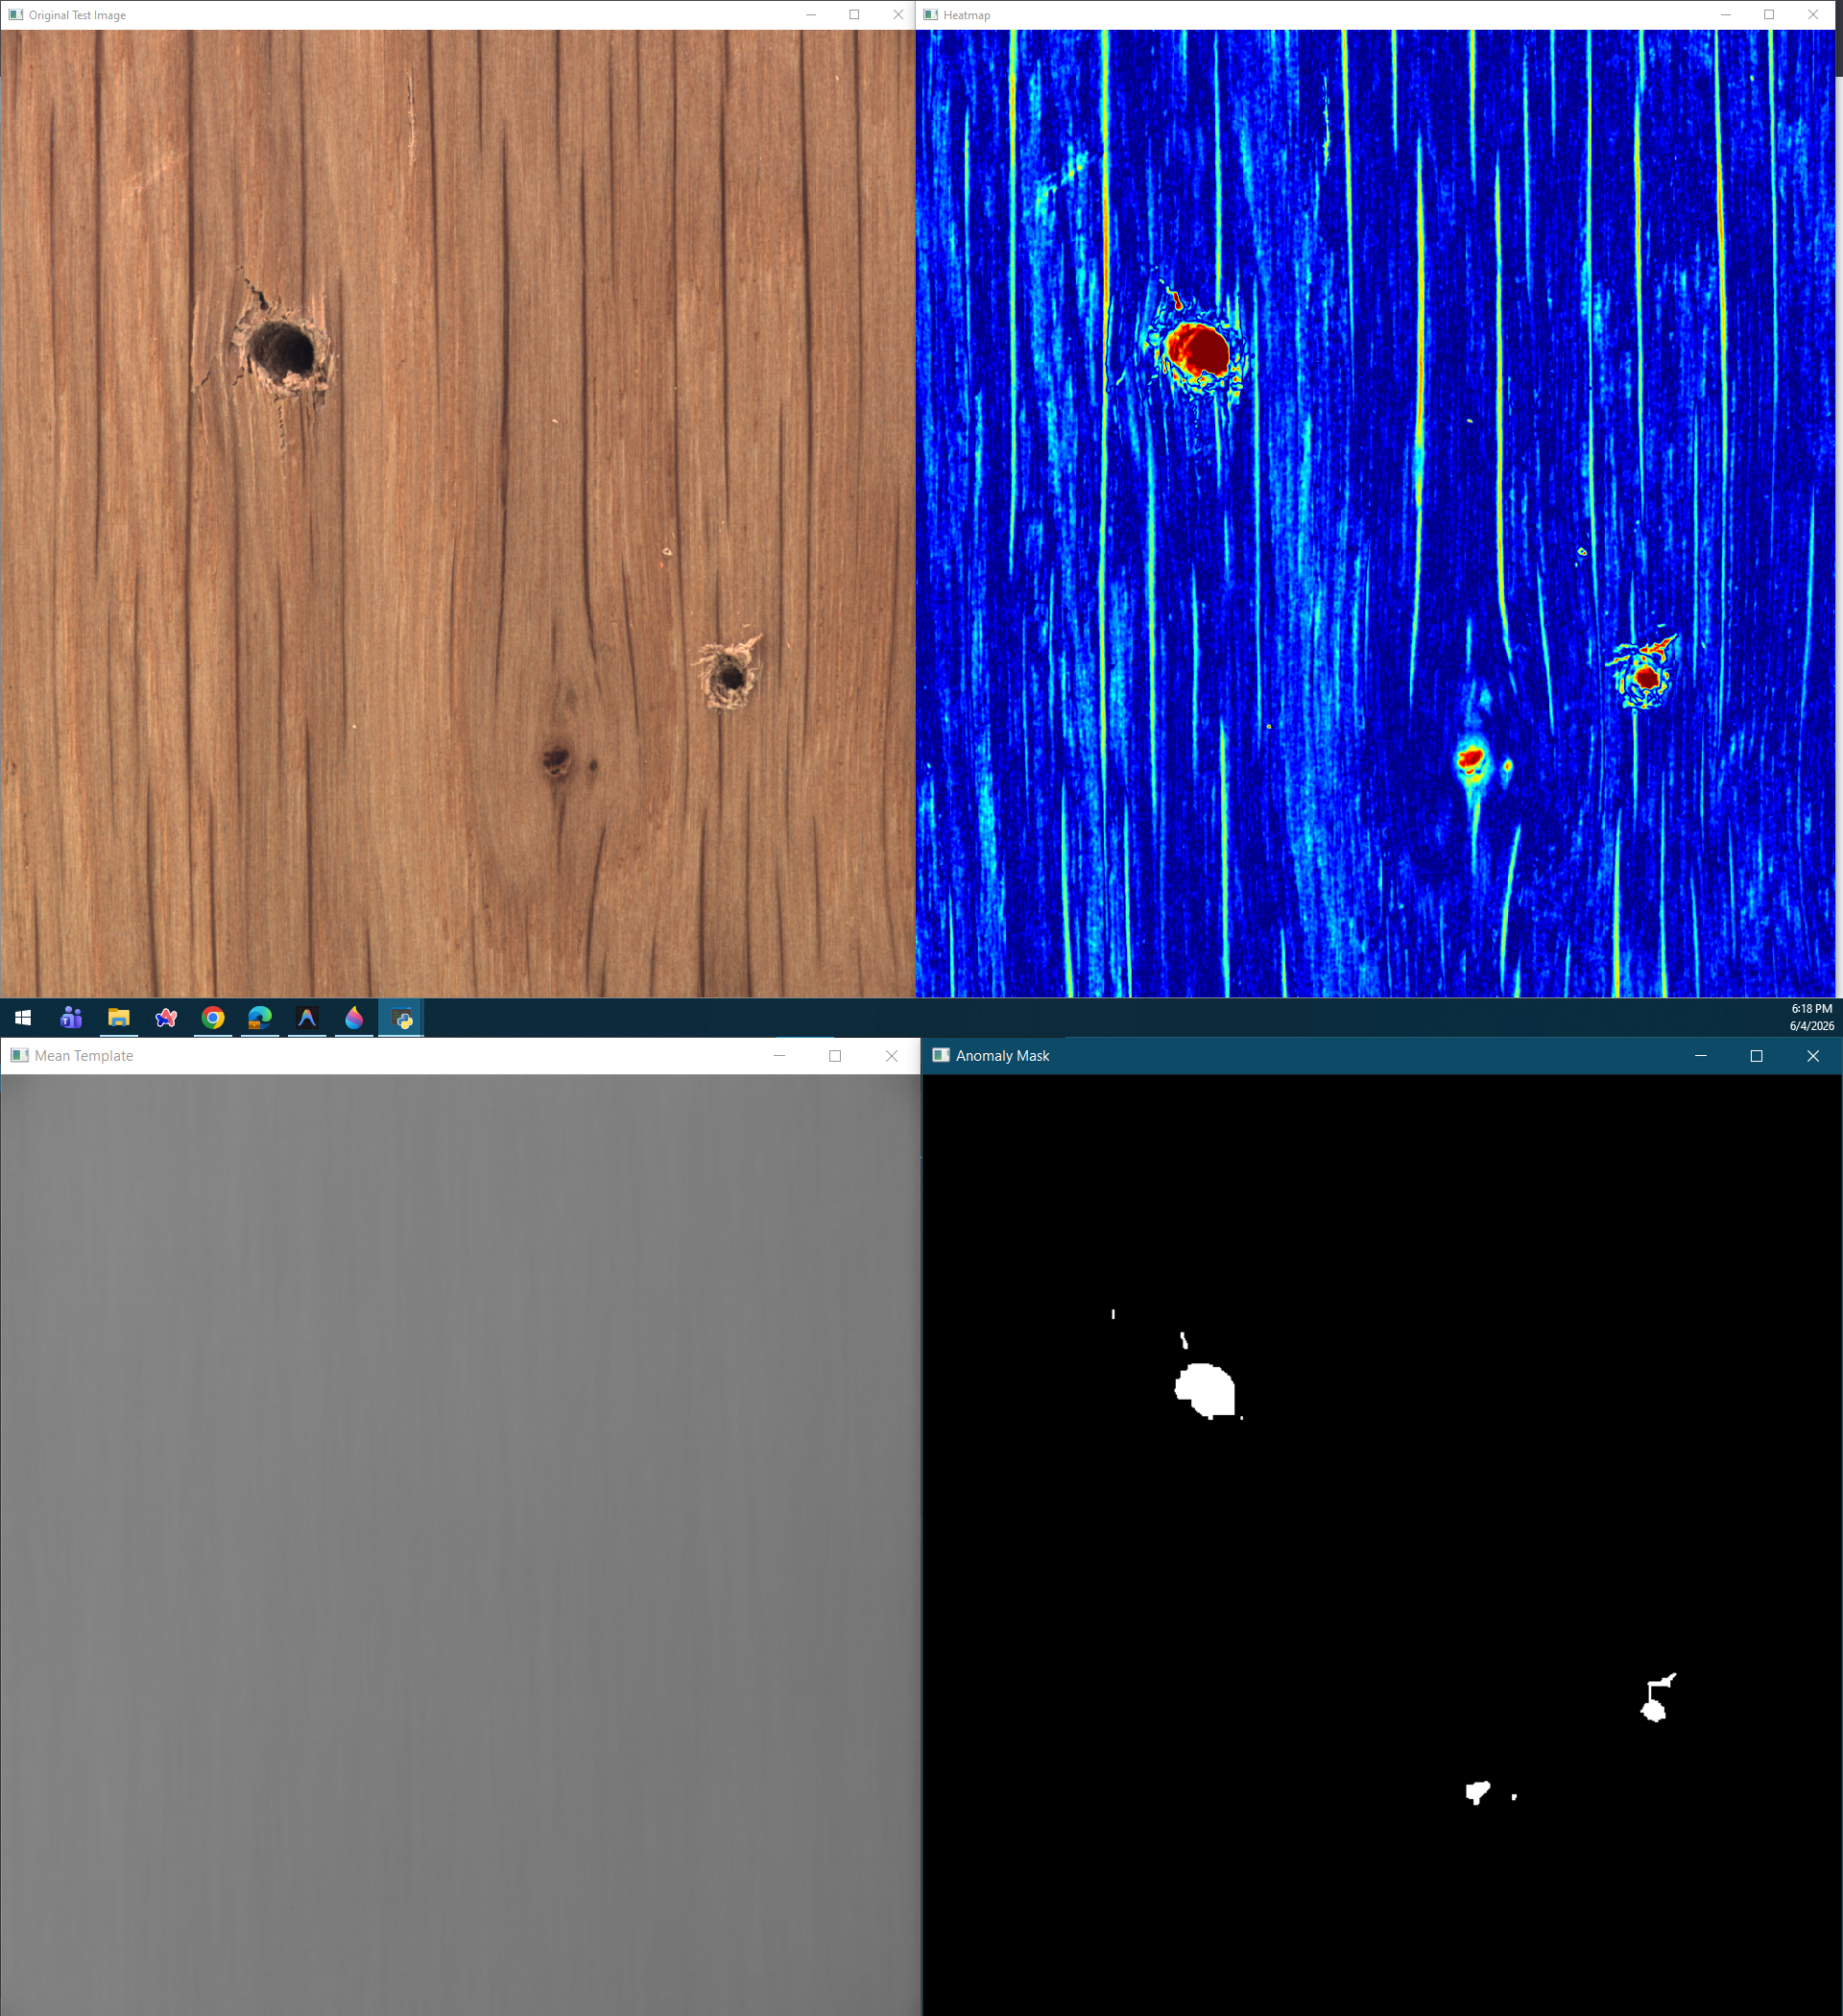
\includegraphics[width=0.8\textwidth]{runtime-images/wood/wood-hole-result0.png}
    \caption{Wood: wood-hole-result0.png}
\end{figure}

\begin{figure}[H]
    \centering
    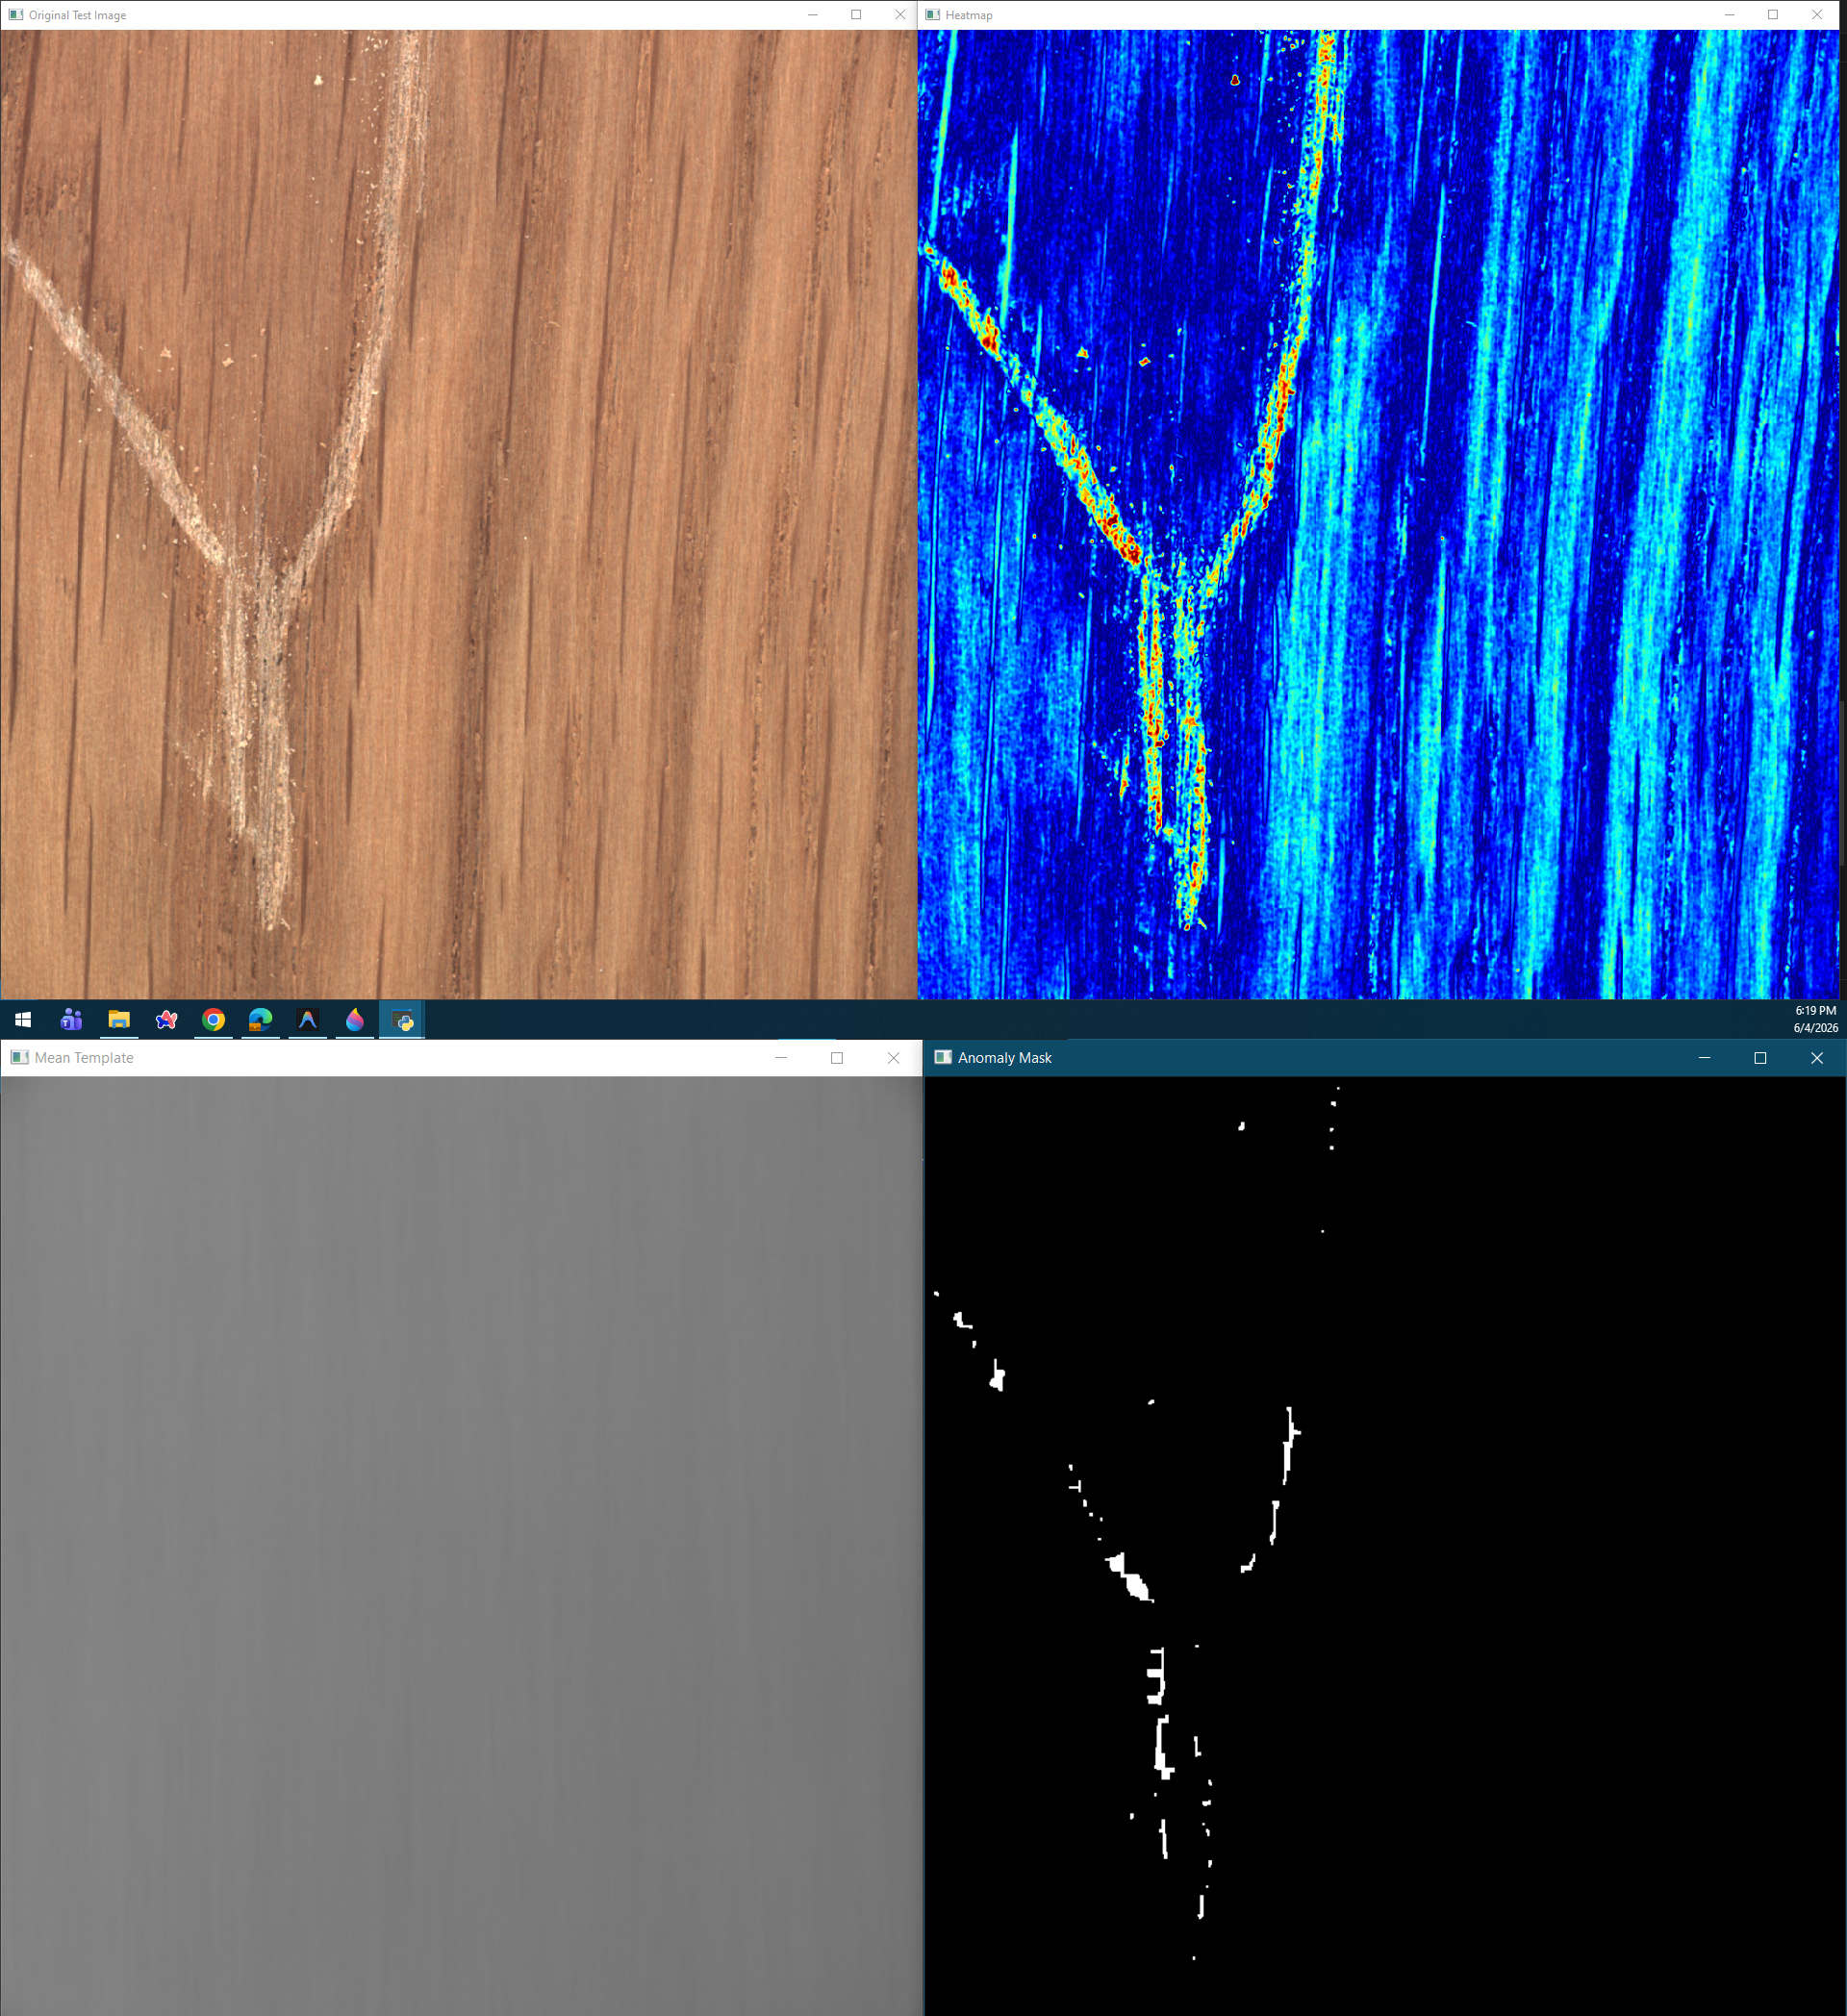
\includegraphics[width=0.8\textwidth]{runtime-images/wood/wood-scratch-result5.png}
    \caption{Wood: wood-scratch-result5.png}
\end{figure}

\subsection{Zipper}
\begin{figure}[H]
    \centering
    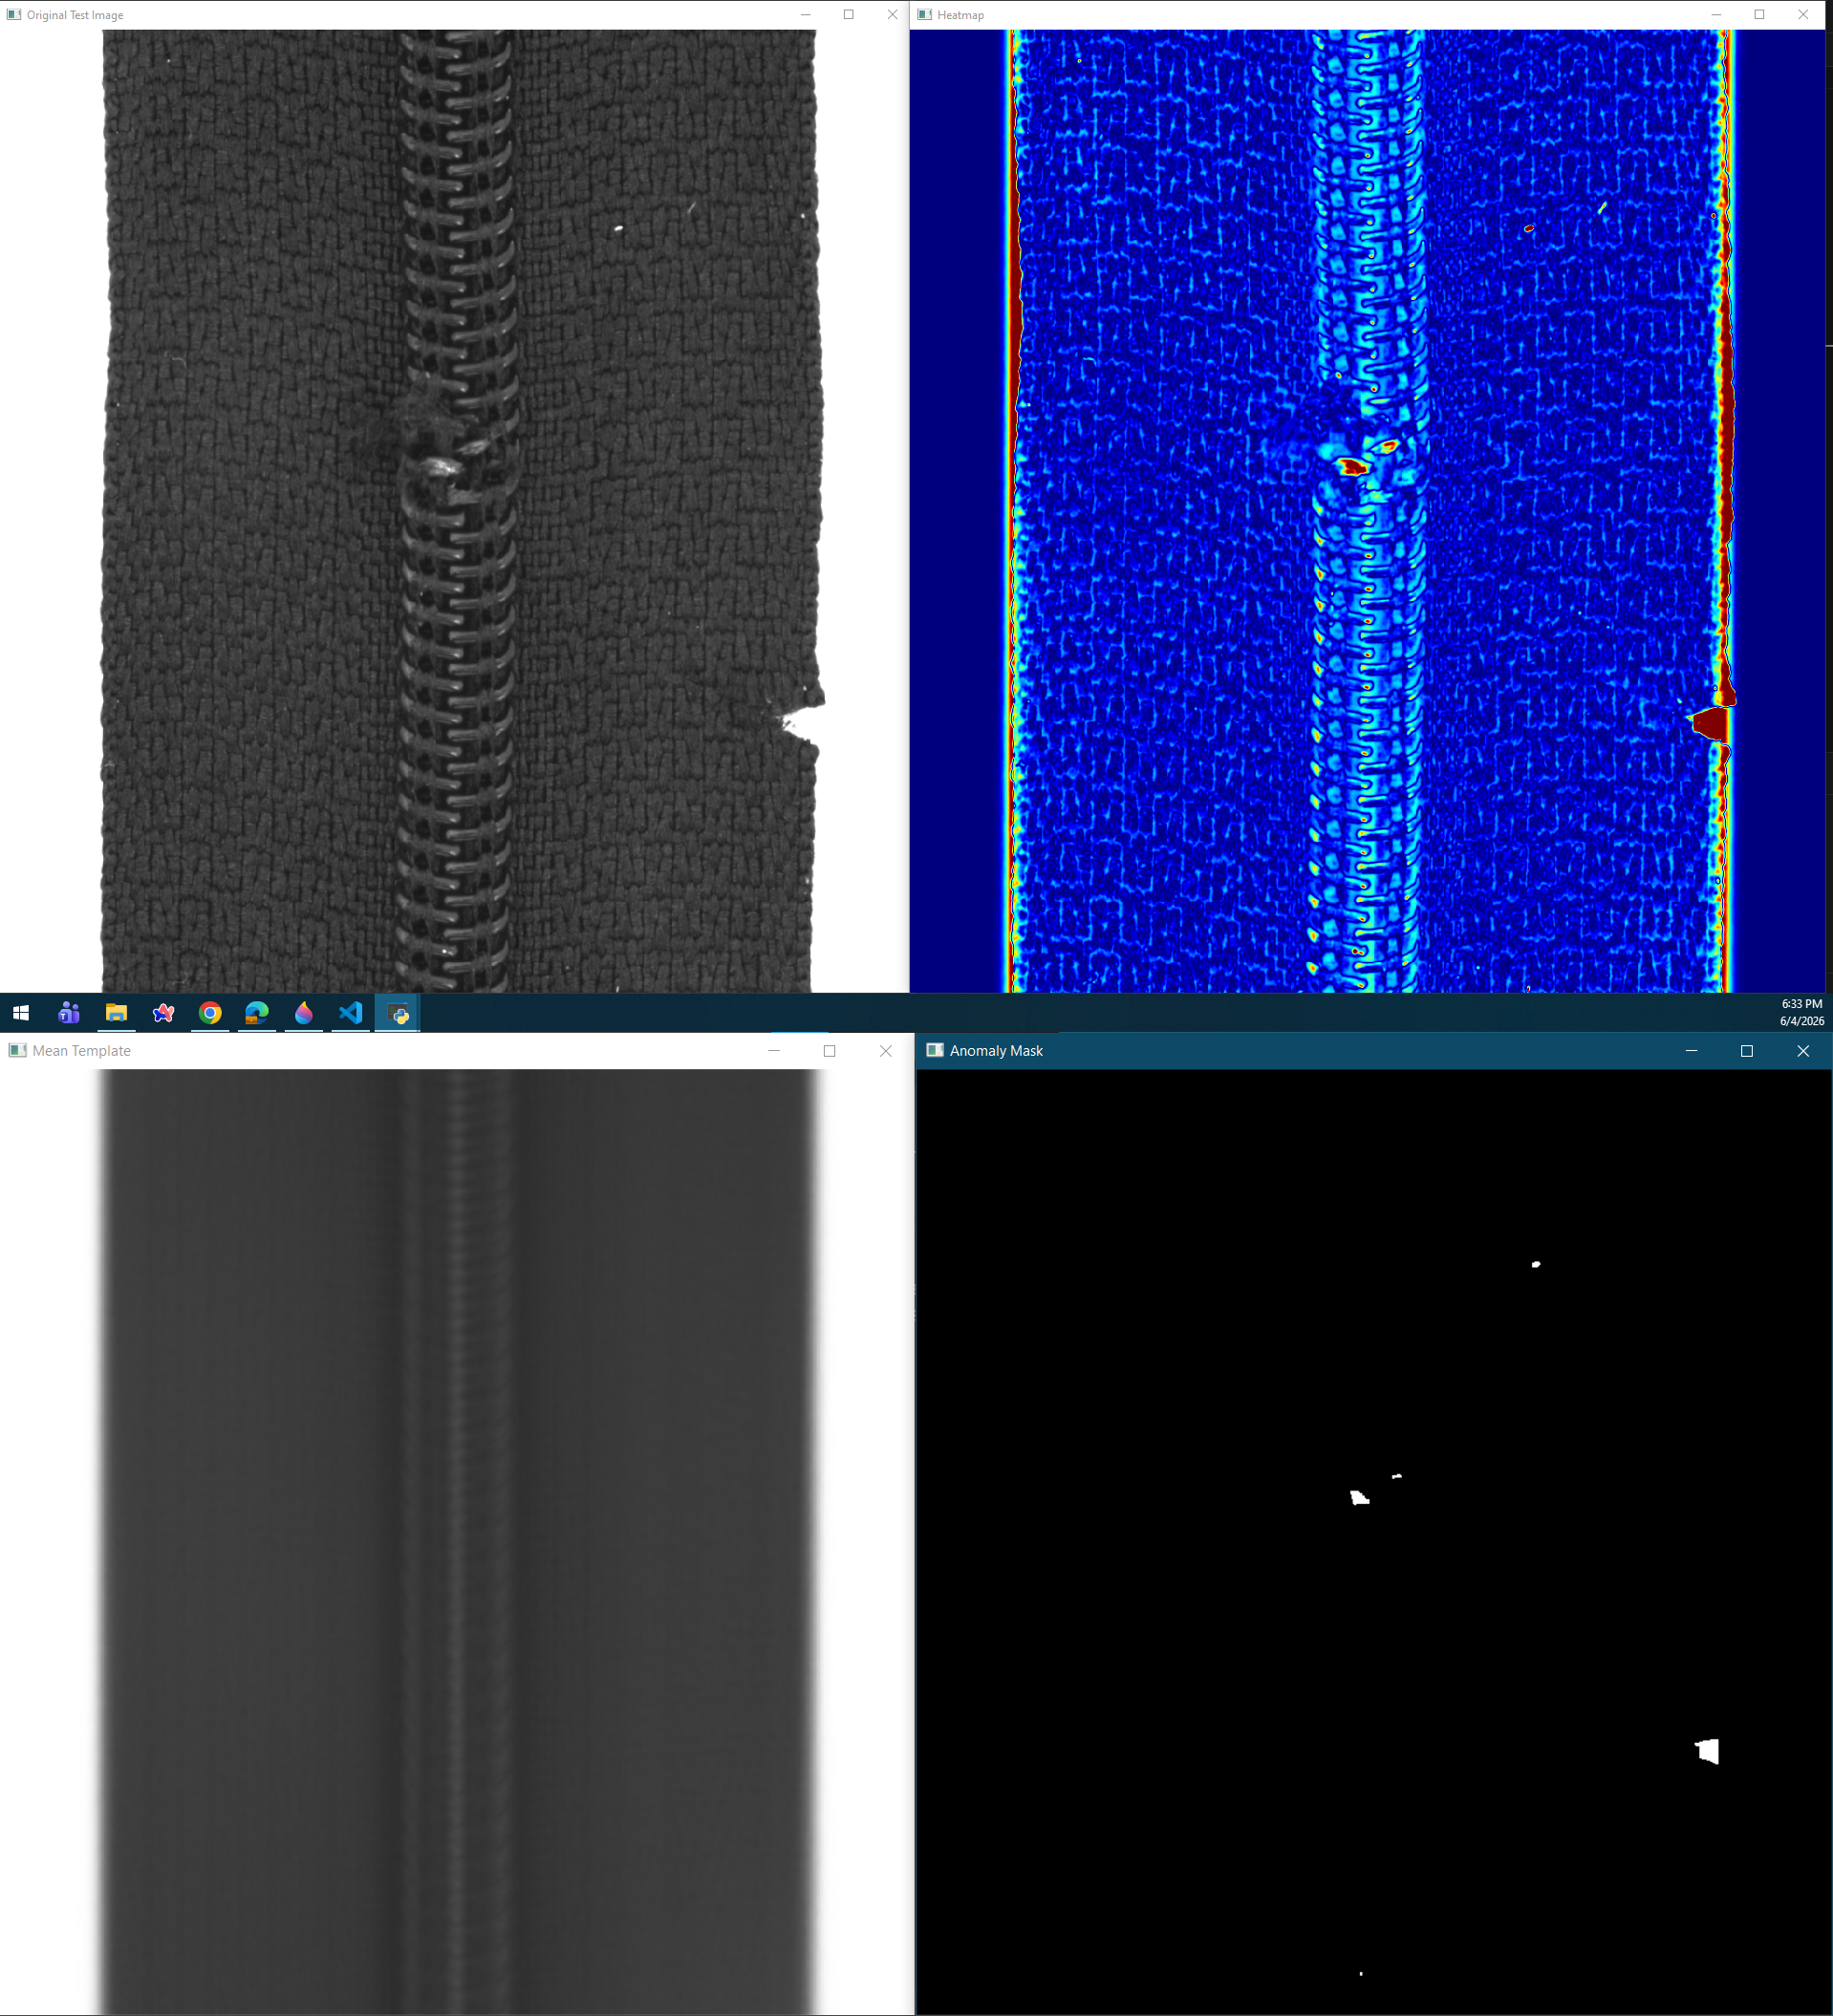
\includegraphics[width=0.8\textwidth]{runtime-images/zipper/zipper-combined-10.png}
    \caption{Zipper: zipper-combined-10.png}
\end{figure}

\begin{figure}[H]
    \centering
    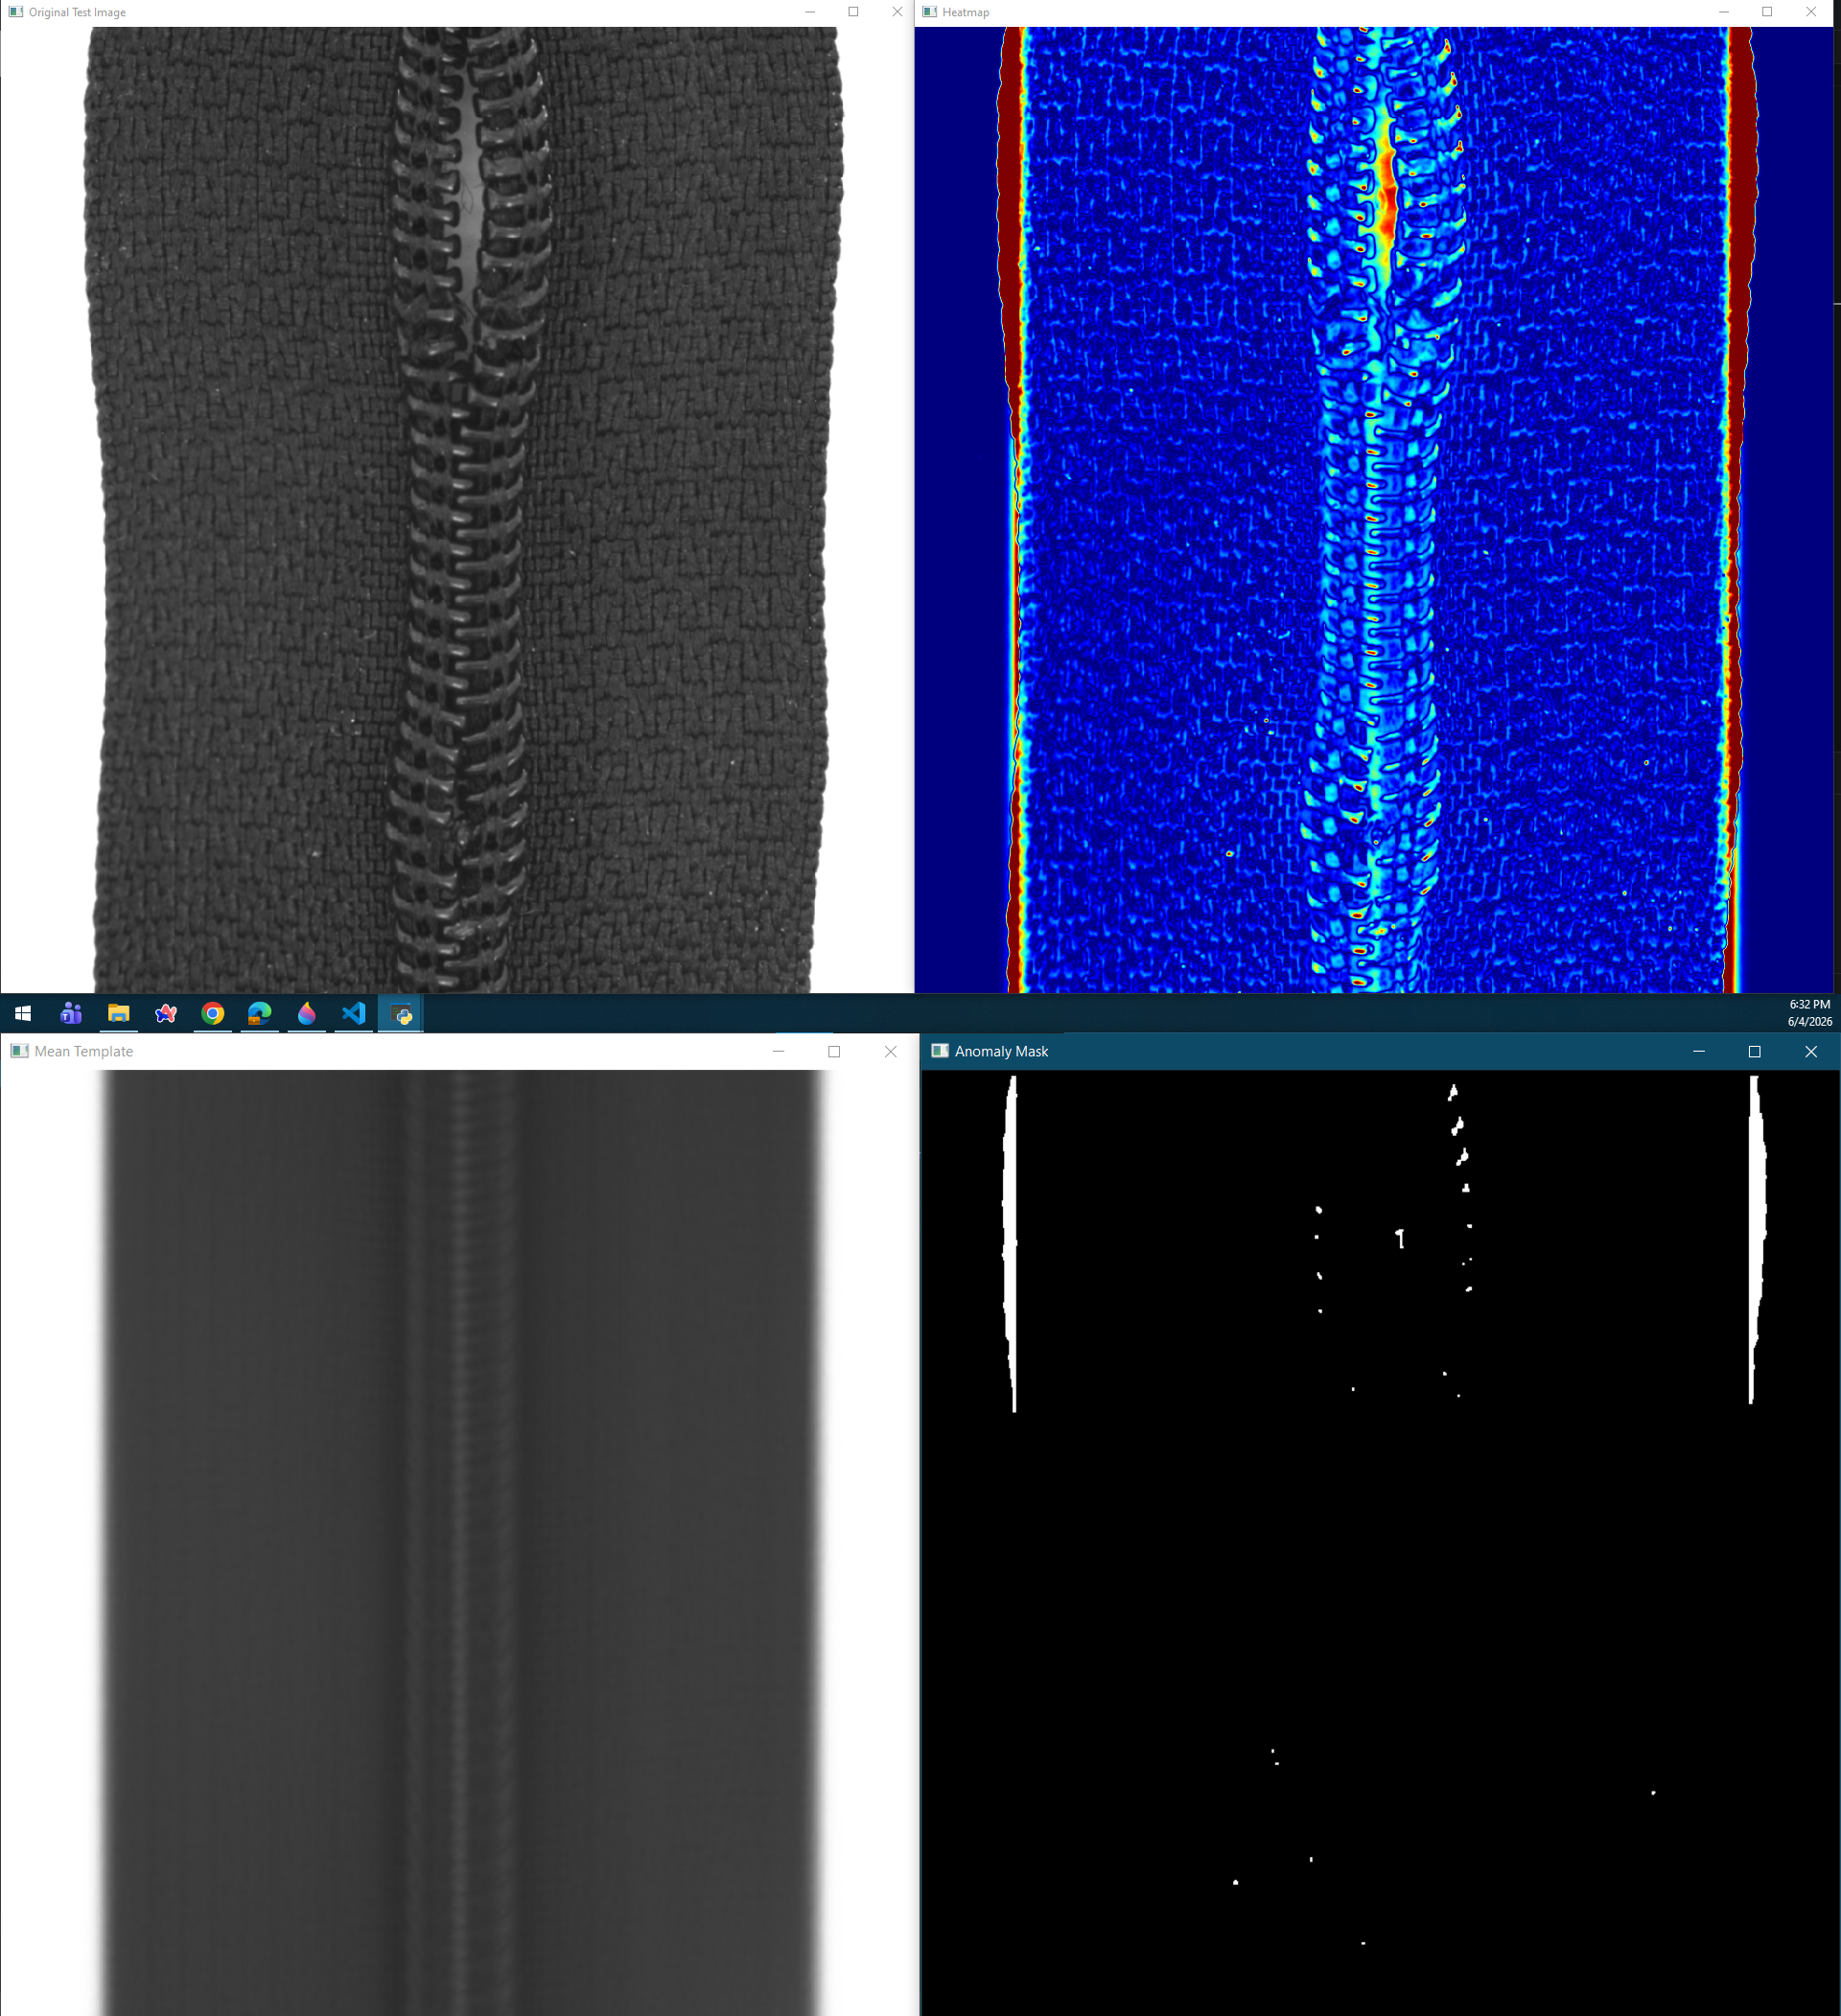
\includegraphics[width=0.8\textwidth]{runtime-images/zipper/zipper-combined-result0.png}
    \caption{Zipper: zipper-combined-result0.png}
\end{figure}

\begin{figure}[H]
    \centering
    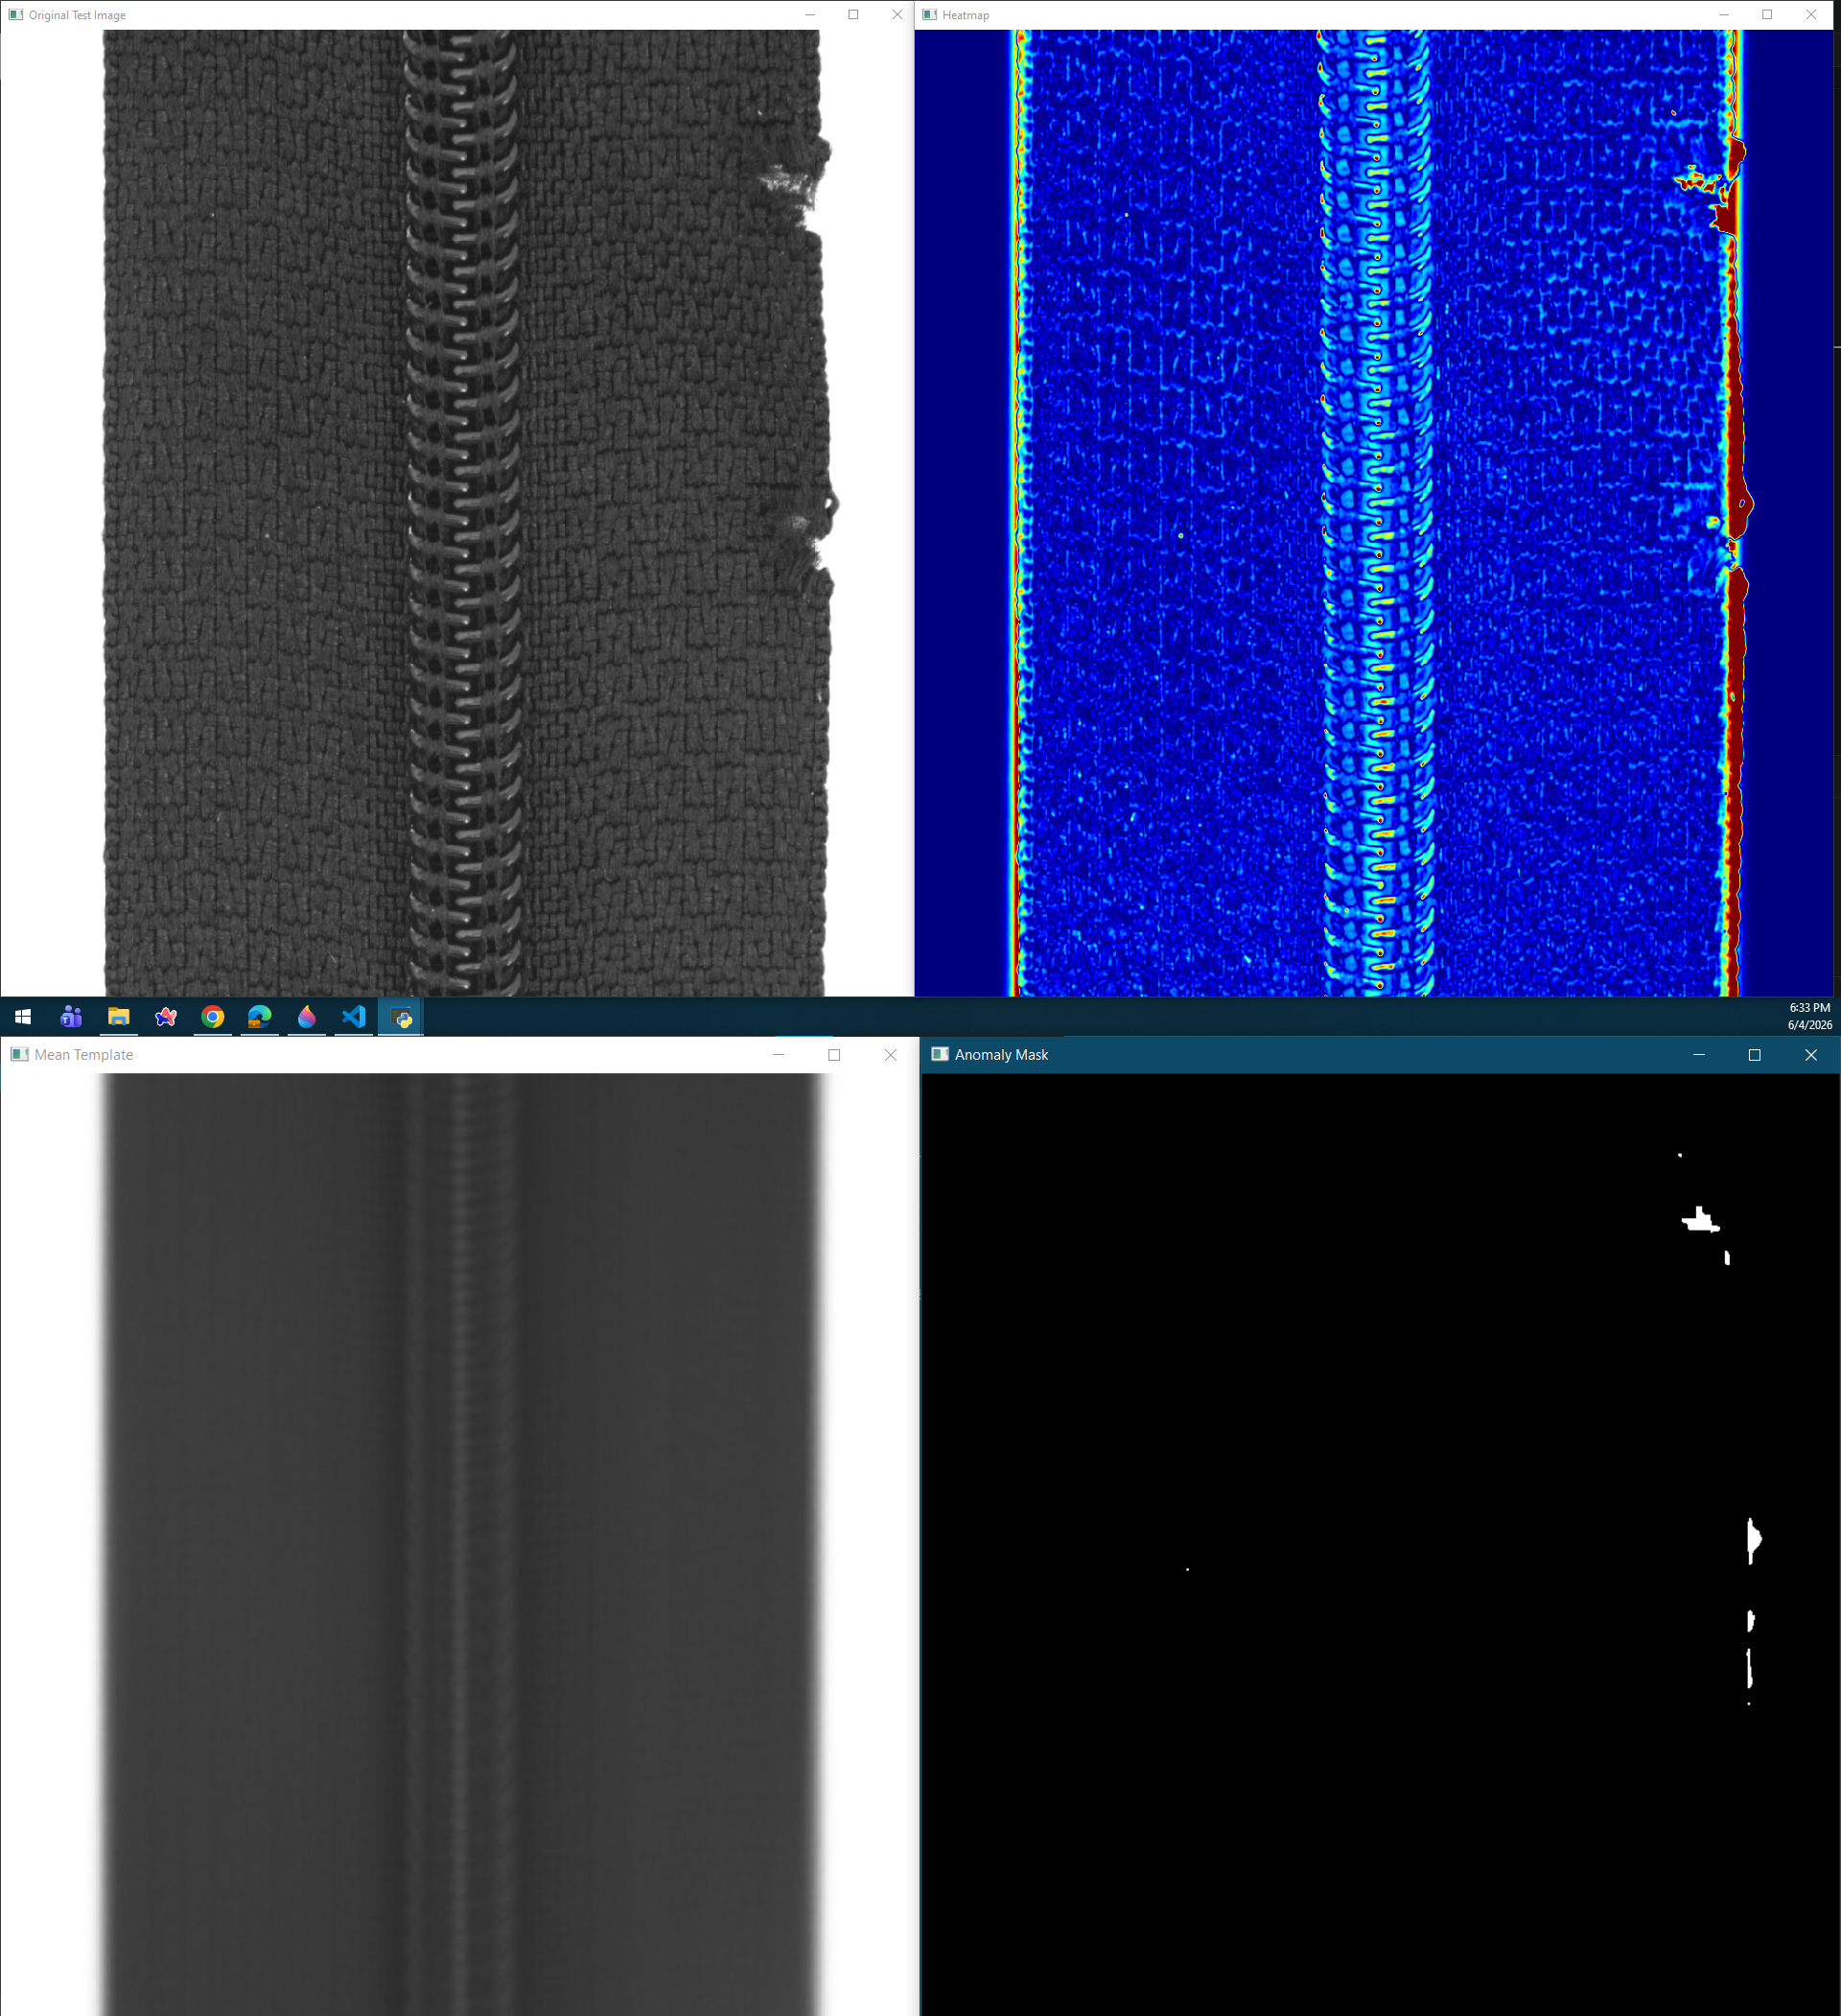
\includegraphics[width=0.8\textwidth]{runtime-images/zipper/zipper-fabric-border-result8.png}
    \caption{Zipper: zipper-fabric-border-result8.png}
\end{figure}

\begin{figure}[H]
    \centering
    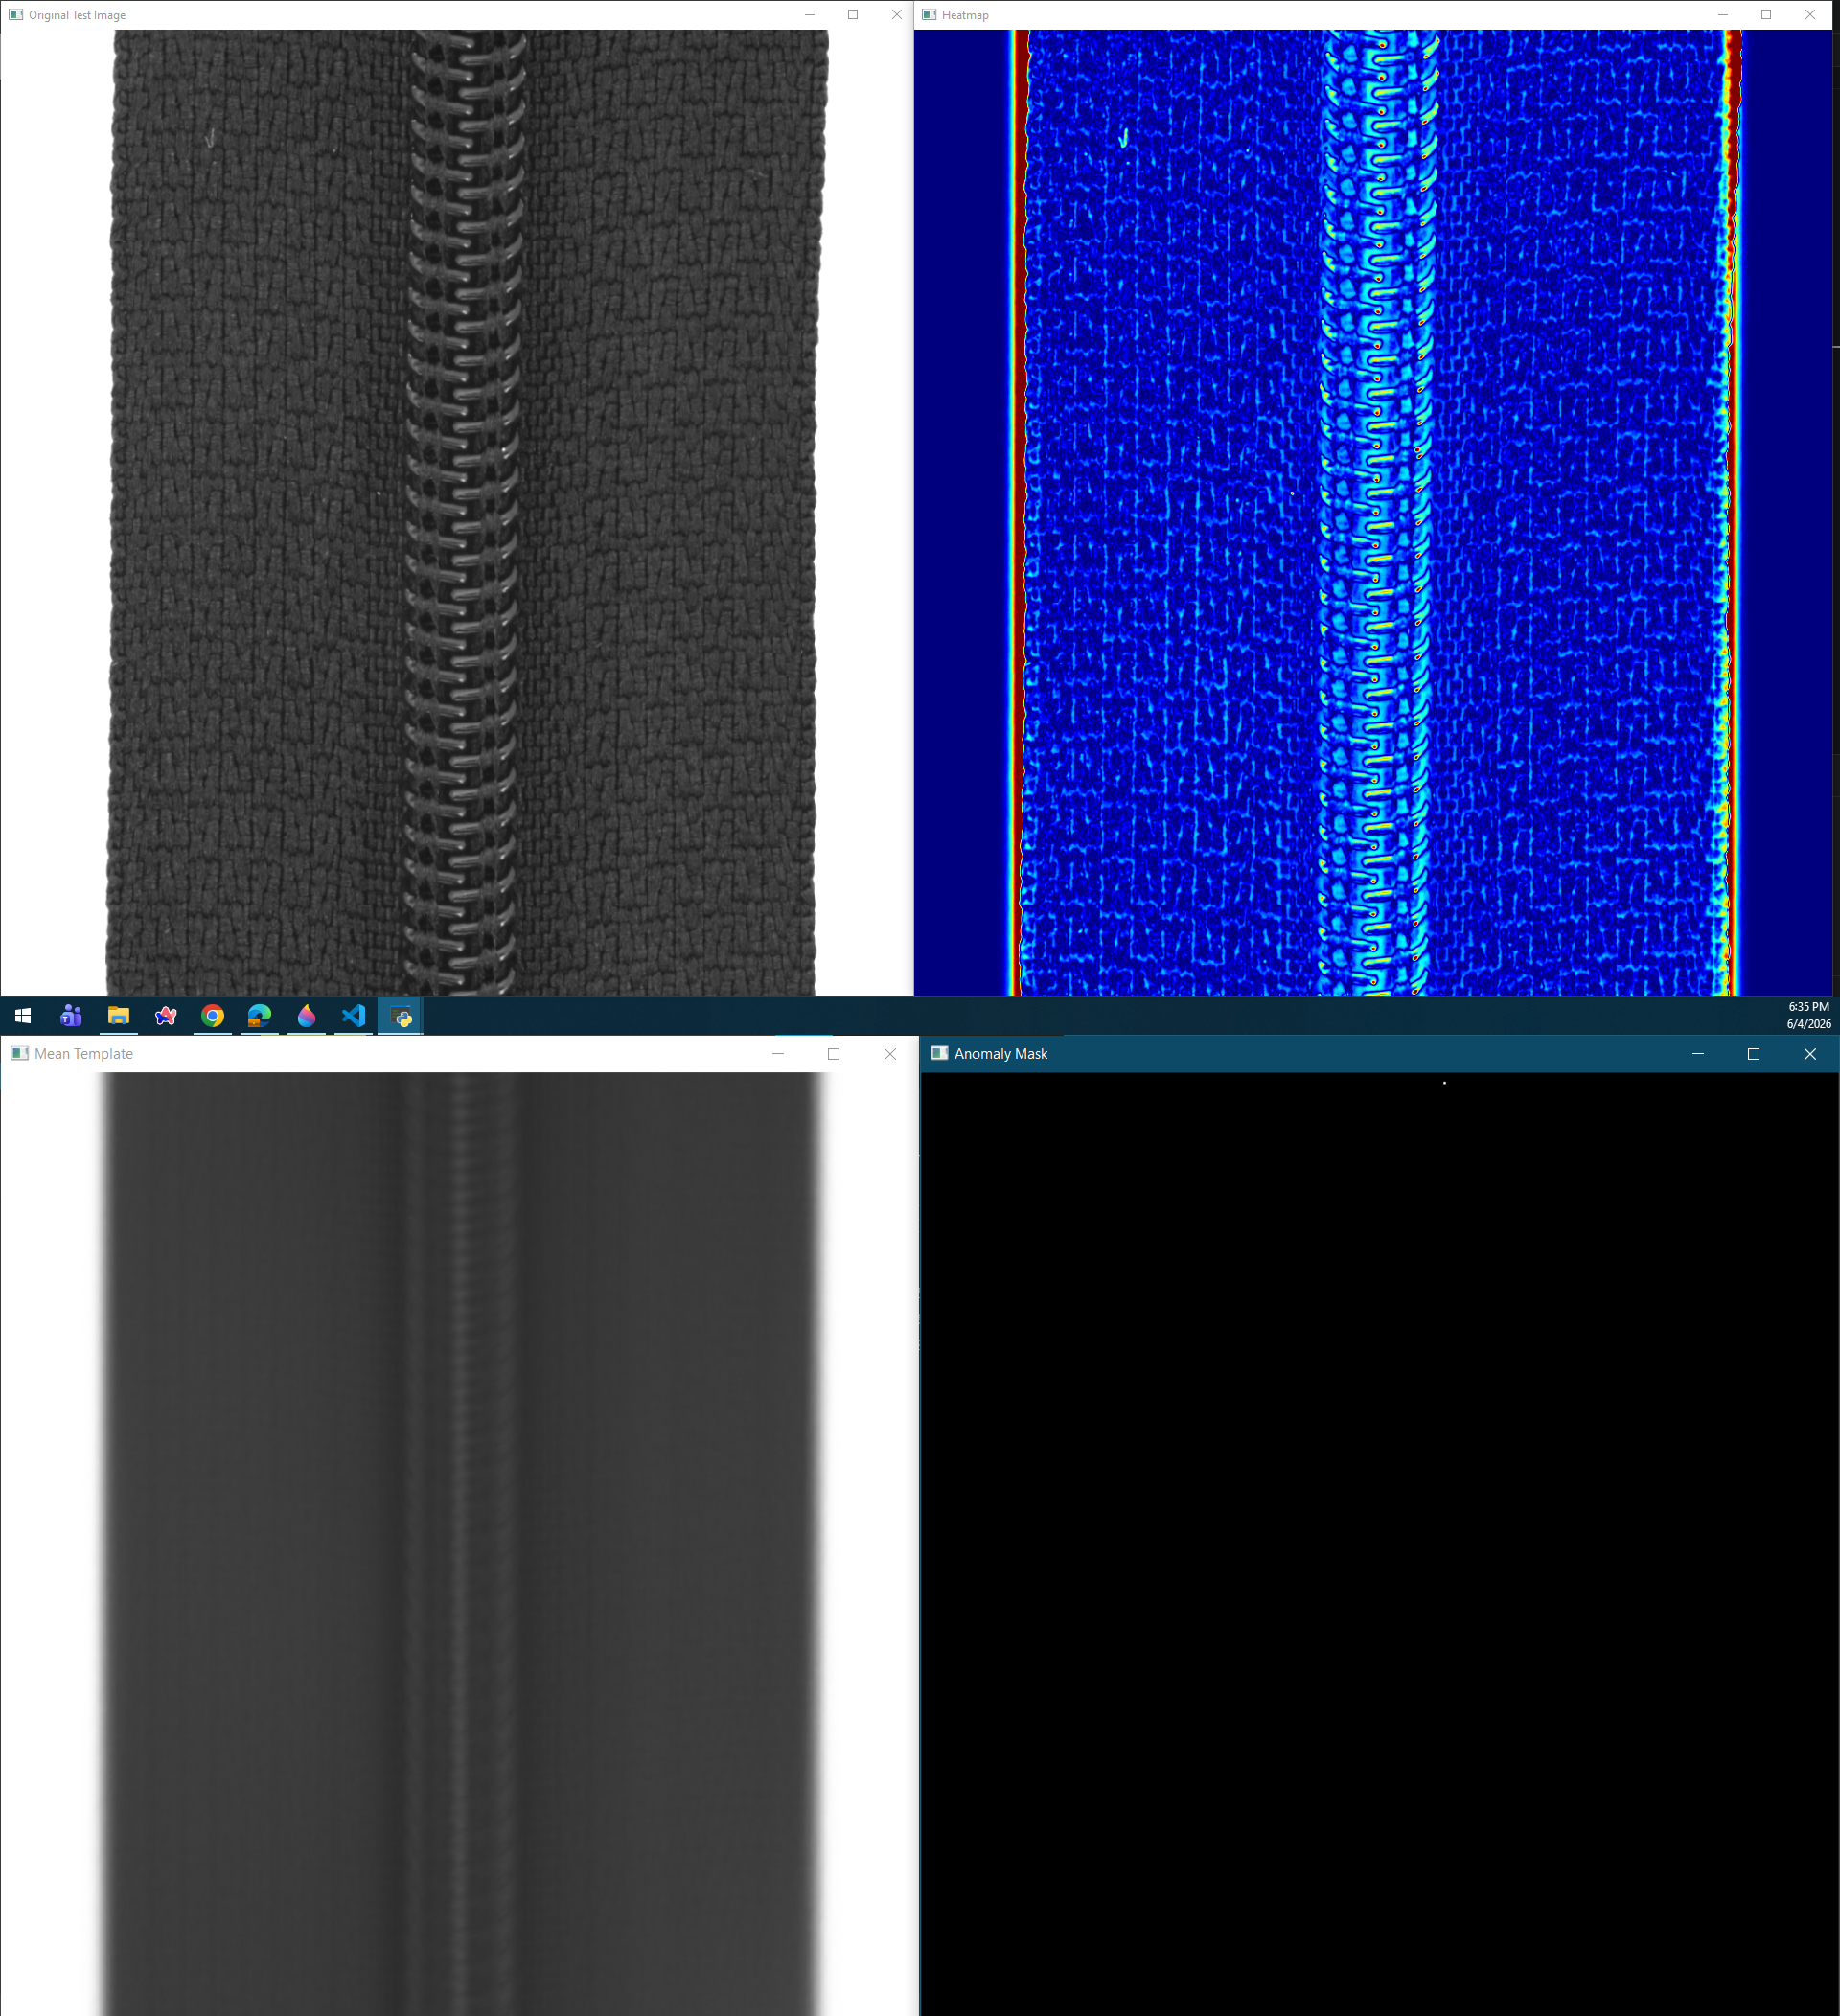
\includegraphics[width=0.8\textwidth]{runtime-images/zipper/zipper-good-result5.png}
    \caption{Zipper: zipper-good-result5.png}
\end{figure}

\end{document}
